\section{Procedimiento}

\noindent Para el desarrollo de las actividades utilice el mismo archivo \texttt{setup\_qube\_rotpen\_lqr.m} empleado en el prelaboratorio.

\subsection*{Actividad 1. Simulación e implementación del control LQR}

Utilice el archivo de Simulink \texttt{act1\_real\_vs\_sim\_qube\_bal\_lqr.slx}. Para esta actividad, considere inicialmente los valores de \textbf{Q} y \textbf{R} utilizados en el prelaboratorio. Sin embargo, dichas ganancias no necesariamente cumplirán con las especificaciones de desempeño durante la implementación real, debido a diferencias entre el modelo simulado y el comportamiento físico del sistema.

Considere una señal de referencia para $\theta$ con forma de onda cuadrada, frecuencia de \textbf{0.1 Hz} y amplitud de \textbf{45 grados}. Utilice un tiempo de simulación e implementación de \textbf{40s}. Las especificaciones de control requeridas son: porcentaje de sobreimpulso $< 5\%$, tiempo de establecimiento $< 3$ s y error en estado estable $\pm 2^\circ$.

\begin{figure}[H]
    \centering
    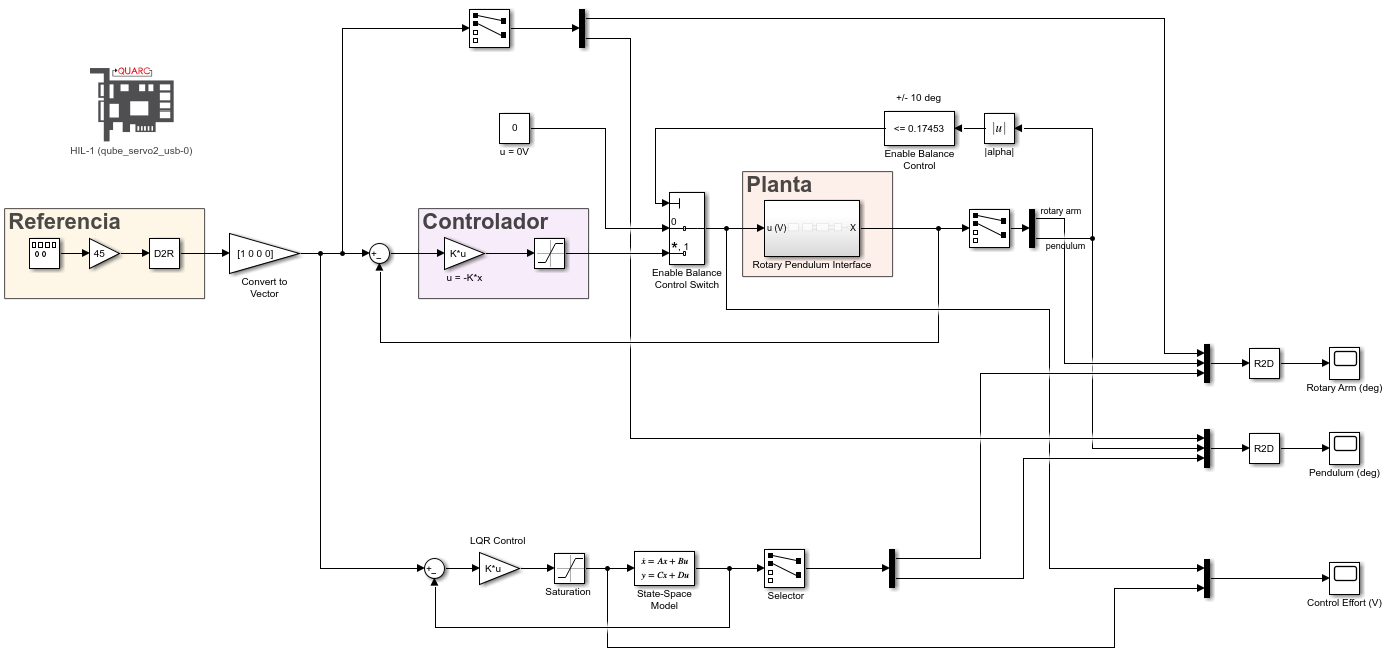
\includegraphics[width=\textwidth]{images/simulink_act1.png}
    \caption{Diagrama de bloques de la Actividad 1 en Simulink.}
    \label{fig:actividad1_diagrama}
\end{figure}

Emplee las matrices de ponderación \textbf{Q} y \textbf{R} del prelaboratorio, o las que hayan funcionado correctamente en simulación, y obtenga el vector de ganancias \textbf{K} correspondiente. Con estos valores, realice tanto la simulación como la implementación en el equipo real.

\noindent Las matrices de ponderación empleadas inicialmente fueron:

\begin{equation}
Q = 
\begin{bmatrix}
100 & 0 & 0 & 0 \\
0 & 100 & 0 & 0 \\
0 & 0 & 27 & 0 \\
0 & 0 & 0 & 10
\end{bmatrix}, \qquad 
R = 7
\end{equation}

\noindent A partir de estas matrices se obtuvo el siguiente vector de ganancias:

\begin{equation}
K = \begin{bmatrix} -3.7796 & 82.9411 & -3.3082  & 6.3191 \end{bmatrix}
\end{equation}

\noindent A continuación se presentan las gráficas comparativas entre simulación e implementación:

% --- Control del brazo rotatorio: sim vs real ---
\begin{figure}[H]
    \centering
    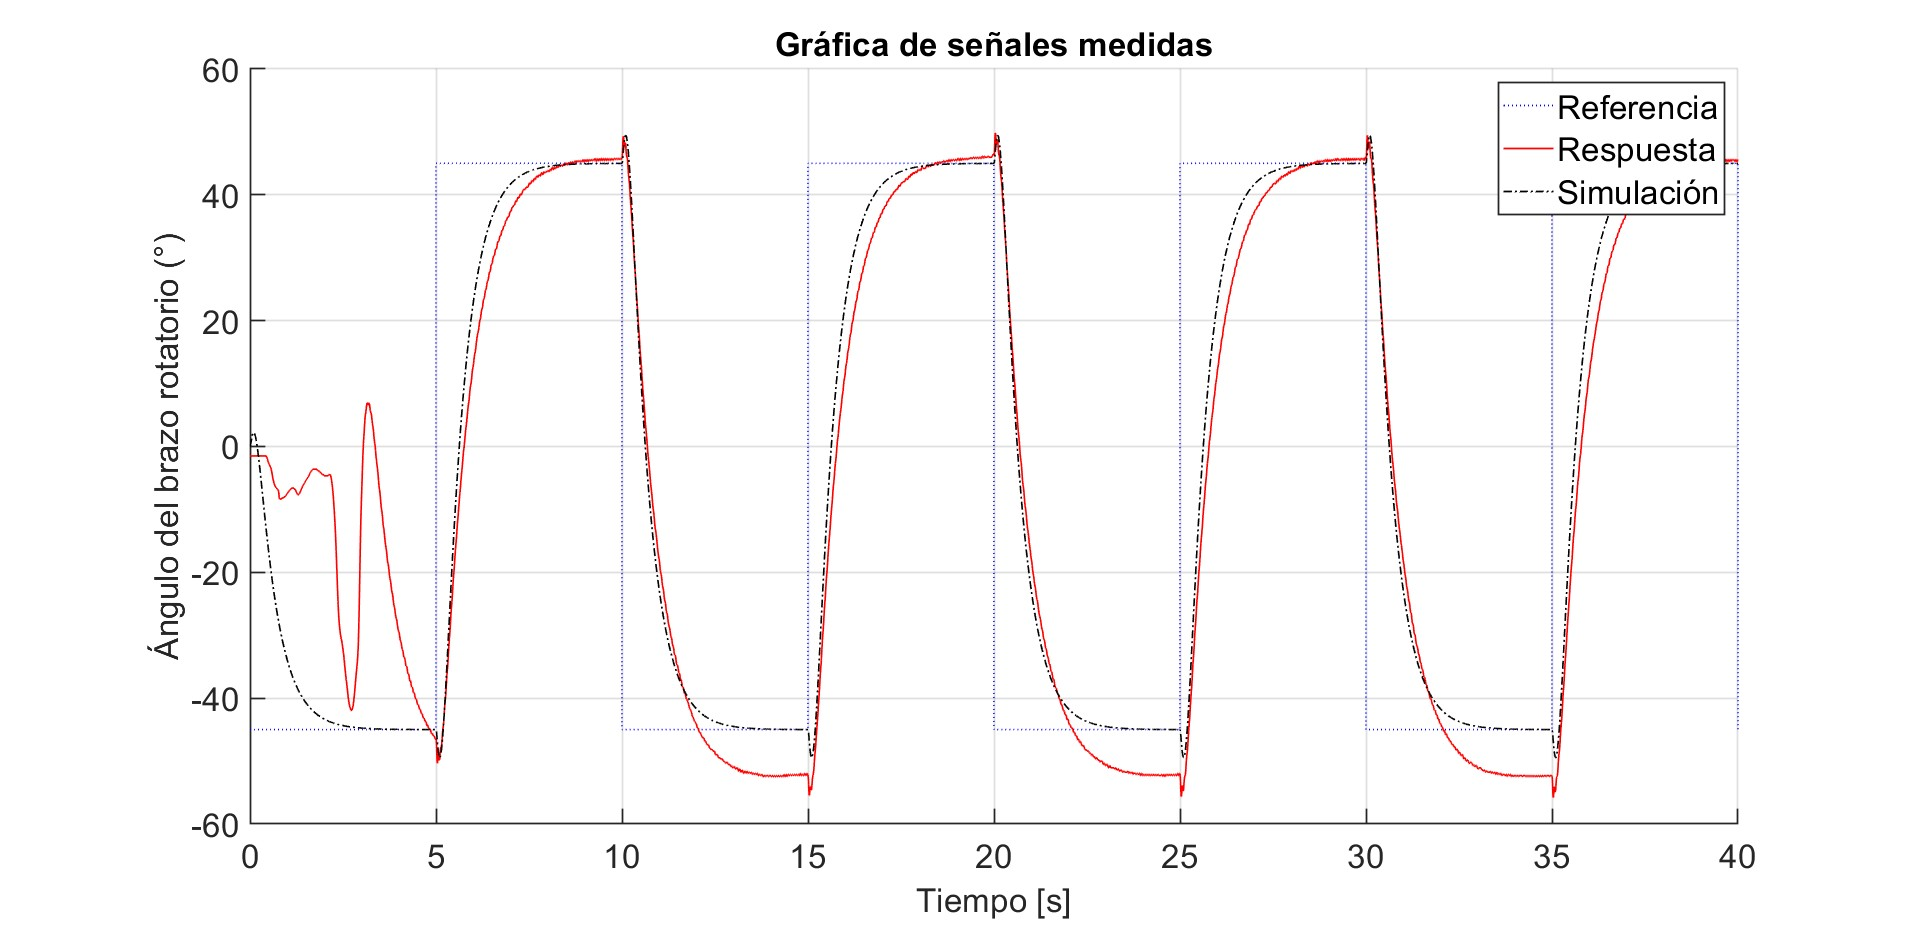
\includegraphics[width=0.85\textwidth]{images/Figura_3.jpg}
    \caption{Control del brazo rotatorio: $\theta$ vs. $\theta_{\text{deseado}}$, comparación entre simulación e implementación.}
    \label{fig:act1_theta_sim_vs_real}
\end{figure}
\noindent Se observa que la respuesta simulada sigue de manera ideal la referencia cuadrada, mientras que la implementación real presenta diferencias debidas a fricción, ruido de los sensores y dinámicas no modeladas del sistema físico.

% --- Control del péndulo invertido: sim vs real ---
\begin{figure}[H]
    \centering
    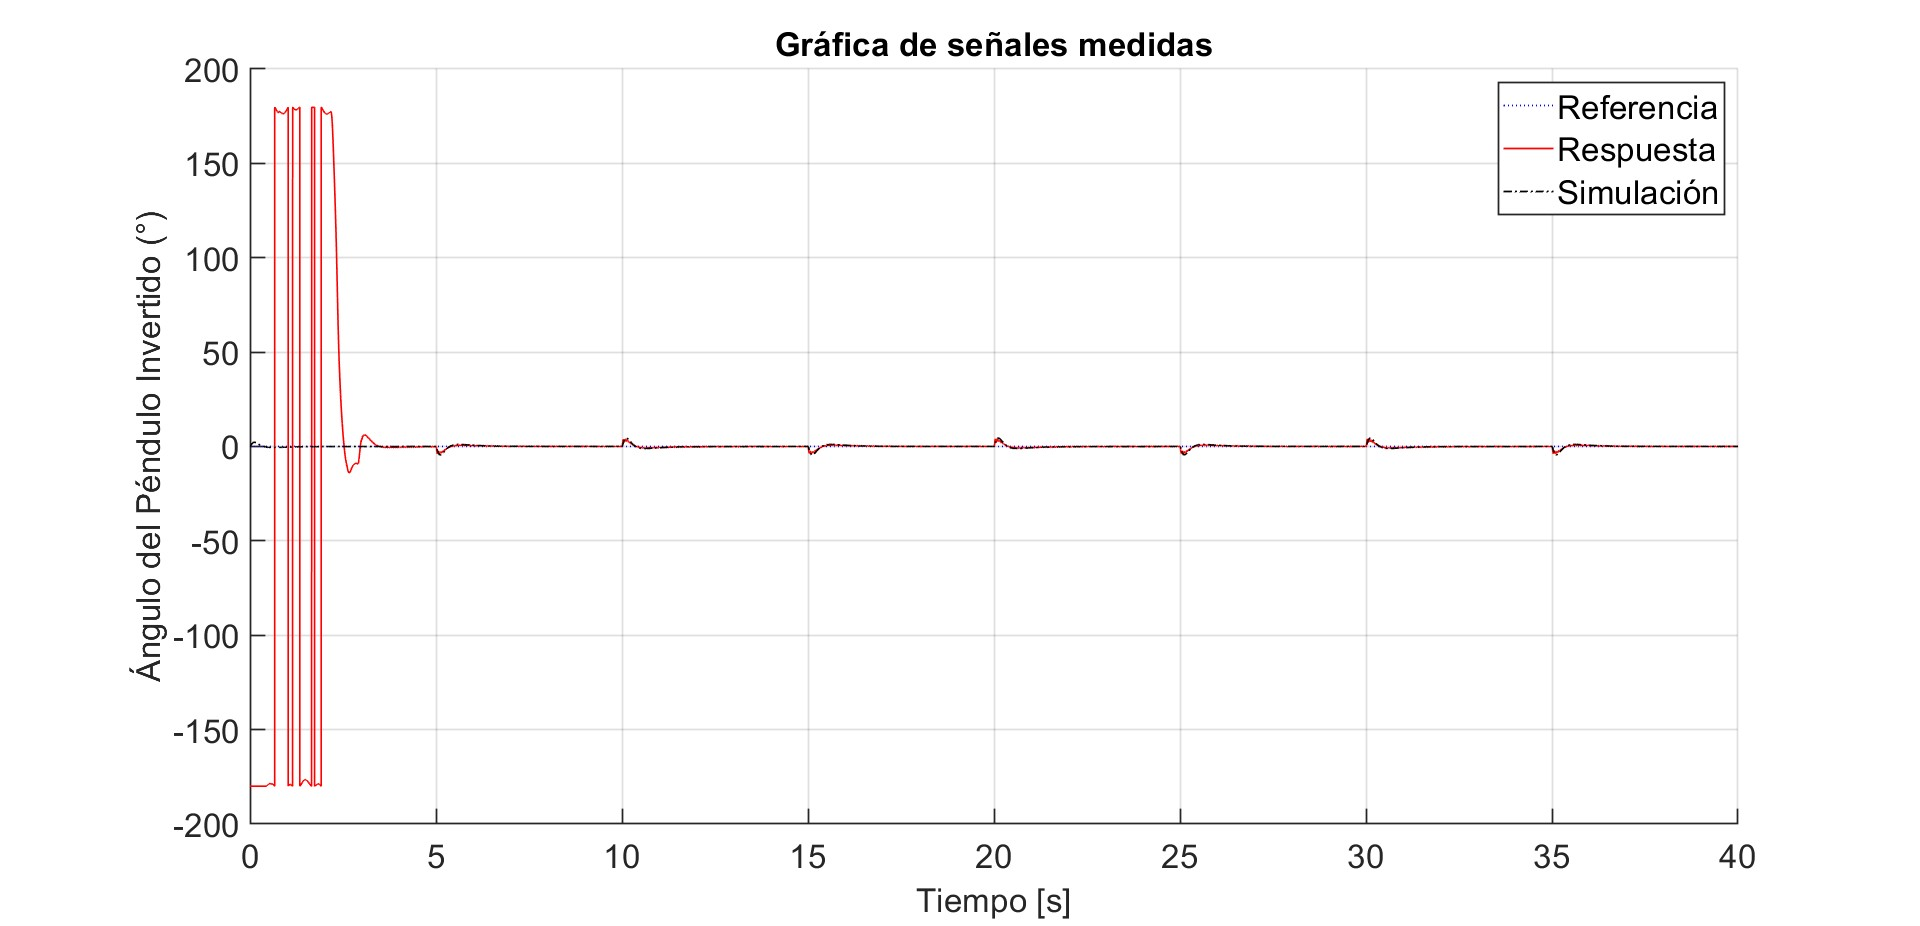
\includegraphics[width=0.85\textwidth]{images/Figura_4.jpg}
    \caption{Control del péndulo invertido: $\alpha$ vs. $\alpha_{\text{deseado}}$, comparación entre simulación e implementación.}
    \label{fig:act1_alpha_sim_vs_real}
\end{figure}
\noindent En simulación, el péndulo se mantiene en la posición invertida ($\alpha_{\text{deseado}} \approx 0$ rad) con oscilaciones prácticamente nulas. En implementación real, $\alpha$ se mantiene acotado dentro de un rango pequeño alrededor de la referencia, aunque con oscilaciones de mayor amplitud debido al ruido de medición del encoder del péndulo y a las perturbaciones del entorno (vibración mecánica del módulo).
% --- Esfuerzo de control: voltaje sim vs real ---
\begin{figure}[H]
    \centering
    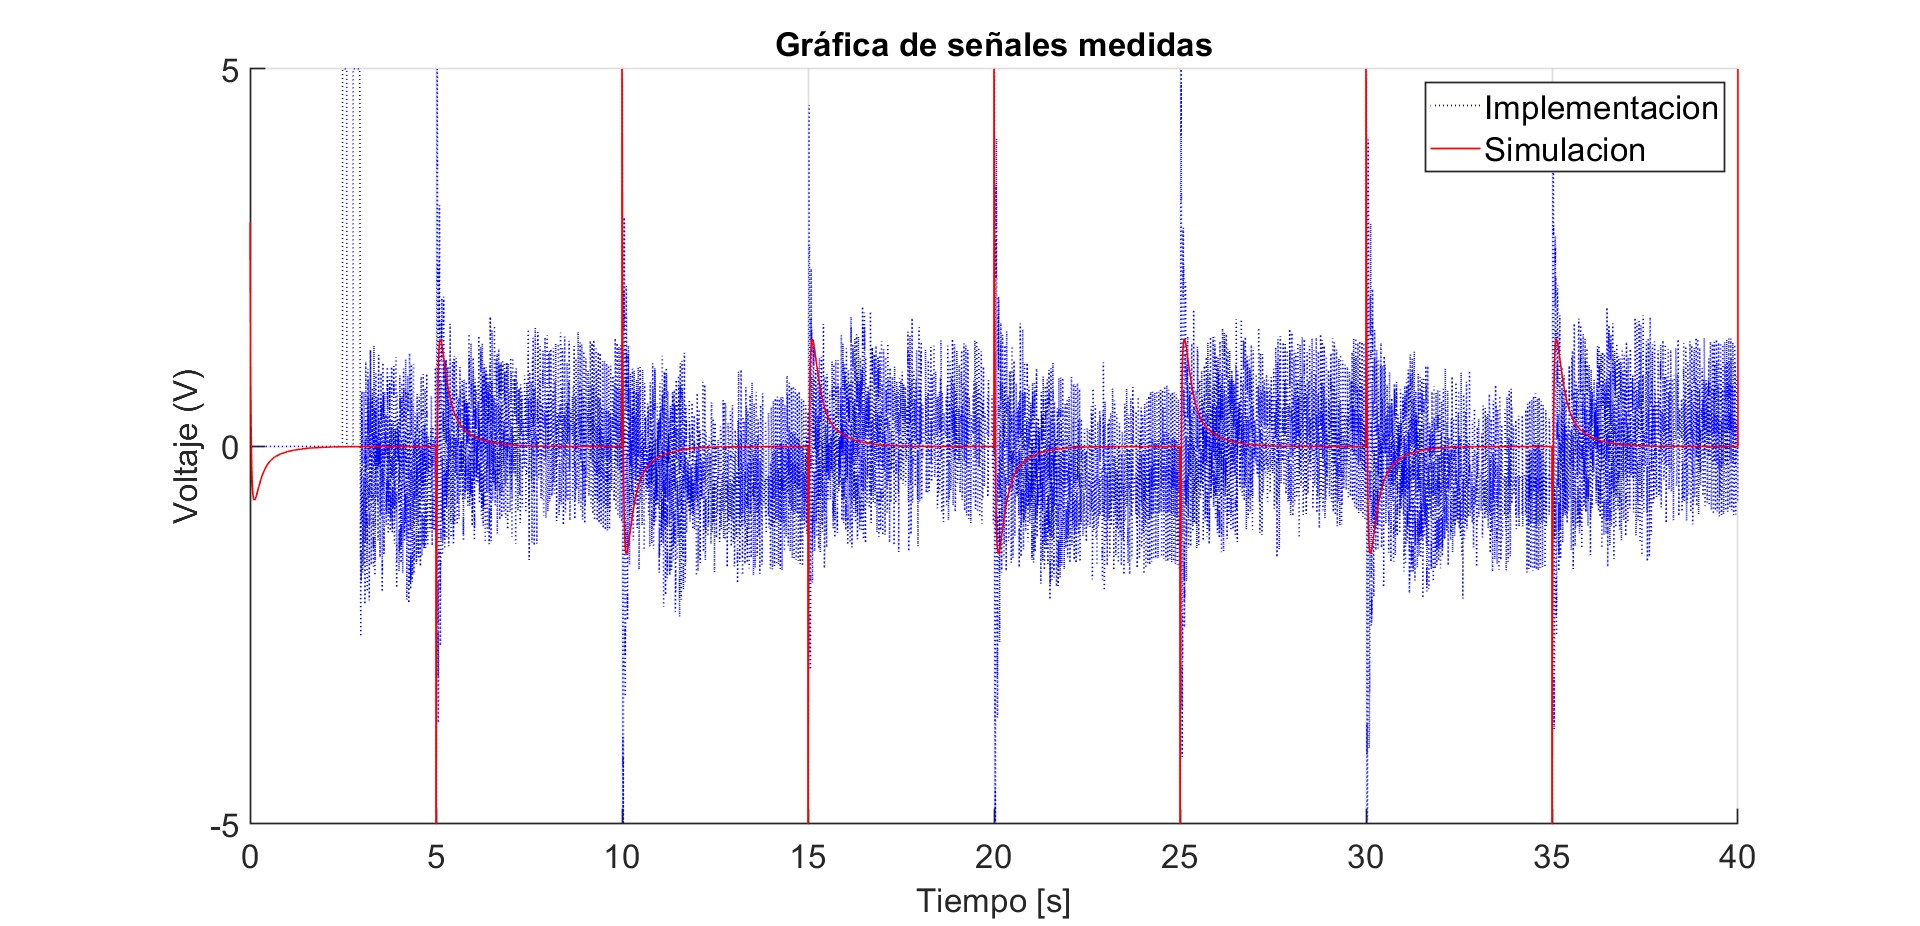
\includegraphics[width=0.85\textwidth]{images/Figura_5.jpg}
    \caption{Esfuerzo de control: voltaje $V_m$, comparación entre simulación e implementación.}
    \label{fig:act1_voltaje_sim_vs_real}
\end{figure}
\noindent El voltaje en simulación resulta más suave, mientras que en implementación presenta mayor actividad y picos asociados a la corrección continua de perturbaciones y al ruido del sistema real.


\noindent En simulación, el voltaje $V_m$ presenta una forma limpia y acotada que responde directamente a los cambios de referencia. En implementación real, $V_m$ muestra mayor actividad de alta frecuencia debido a que el controlador corrige continuamente las perturbaciones y el ruido captado por los sensores. La amplitud máxima del voltaje permanece dentro de los límites del actuador, lo que indica que las ganancias seleccionadas no saturan el motor.
Tabla~\ref{tab:act1_desempeno_inicial}.

\begin{table}[H]
\centering
\caption{Parámetros de desempeño del control de $\theta$ con $Q$ y $R$ del prelaboratorio.}
\label{tab:act1_desempeno_inicial}
\renewcommand{\arraystretch}{1.3}
\begin{tabular}{|c|c|c|c|}
\hline
\textbf{Parámetro} & \textbf{Especificación} & \textbf{Obtenido} & \textbf{Cumple} \\\hline
Sobreimpulso          & $< 5\%$  & $0.42\%$  & Sí \\\hline
Tiempo de establecimiento & $< 3$ s  & $2.926$ s & Sí \\\hline
Error en estado estable & $\pm 2°$ & $2.10\%$ & Sí \\\hline
\end{tabular}
\end{table}

Compare los resultados de \textbf{simulación} e \textbf{implementación} a partir de las gráficas obtenidas de $\theta$, $\alpha$ y voltaje, así como de los parámetros de desempeño del control de $\theta$ (\textbf{porcentaje de sobreimpulso}, \textbf{tiempo de establecimiento} y \textbf{error en estado estable}). Indique si la implementación real reproduce el comportamiento esperado en simulación y explique las principales diferencias observadas. \\
\noindent A partir de las gráficas y la Tabla~\ref{tab:act1_desempeno_inicial}, la implementación real \textbf{reproduce satisfactoriamente} el comportamiento esperado en simulación. Los tres parámetros de desempeño cumplen las especificaciones: sobreimpulso de $0.42\%$ (muy por debajo del $5\%$ exigido), tiempo de establecimiento de $2.926$ s (dentro del límite de $3$ s) y error en estado estable de $2.10\%$ (cercano al límite de $\pm 2^\circ$). Las diferencias menores entre simulación e implementación se atribuyen a la fricción no modelada, el ruido de los encoders y las dinámicas eléctricas del motor no consideradas en el modelo linealizado.

\noindent Debido a que las matrices de ponderación propuestas inicialmente  cumplieron las especificaciones desde la primera iteración, no fue necesario realizar un proceso adicional de ajuste fino para obtener nuevas ganancias óptimas. En otras palabras, el primer conjunto de matrices $Q$ y $R$ evaluado produjo directamente un desempeño satisfactorio tanto en simulación como en implementación real. Por ello, se considera que estas matrices corresponden al ajuste óptimo empleado en las actividades siguientes.

\begin{equation}
Q_{\text{optimo}} = 
\begin{bmatrix}
100 & 0 & 0 & 0 \\
0 & 100 & 0 & 0 \\
0 & 0 & 27 & 0 \\
0 & 0 & 0 & 10
\end{bmatrix},
\qquad
R_{\text{optimo}} = 7
\end{equation}

\noindent El vector de ganancias asociado es:

\begin{equation}
K_{\text{optimo}} =
\begin{bmatrix}
-3.7796 & 82.9411 & -3.3082 & 6.3191
\end{bmatrix}
\end{equation}

\noindent Con estas matrices, el brazo sigue la referencia cuadrada cumpliendo las especificaciones de desempeño: sobreimpulso menor al $5\%$, tiempo de establecimiento menor a $3$ s y error en estado estable dentro de $\pm 2^\circ$.

\noindent Asimismo, el péndulo se mantiene estable cerca de la posición invertida con oscilaciones reducidas, mientras que el voltaje aplicado permanece acotado y consistente con las capacidades del actuador, evidenciando un compromiso adecuado entre desempeño y esfuerzo de control.


\subsection*{Actividad 2. Análisis del efecto de variar las matrices Q y R}

Utilice el archivo de Simulink \texttt{act2\_q\_qube\_bal\_lqr.slx}. Considere como valores \textbf{óptimos} $Q_{\text{opt}}$ y $R_{\text{opt}}$,  los valores de \textbf{Q} y \textbf{R} de la Actividad 1 que cumplieron con los parámetros de desempeño en implementación y a partir de ellos implemente los siguientes cuatro casos:

\begin{itemize}
    \item $Q_{\text{mayor}}$ y $R_{\text{opt}}$
    \item $Q_{\text{menor}}$ y $R_{\text{opt}}$
    \item $Q_{\text{opt}}$ y $R_{\text{mayor}}$
    \item $Q_{\text{opt}}$ y $R_{\text{menor}}$
\end{itemize}

Para los casos de \textbf{$Q_{\text{mayor}}$} y \textbf{$Q_{\text{menor}}$}, cambie al menos \textbf{un valor de la diagonal} de la matriz \textbf{Q}; no es necesario modificar todos los elementos diagonales. Para los casos de \textbf{$R_{\text{mayor}}$} y \textbf{$R_{\text{menor}}$}, modifique el valor de \textbf{R} con respecto al caso óptimo. En esta actividad, los cuatro casos evaluados \textbf{no necesariamente deben cumplir} con las especificaciones de desempeño exigidas en la Actividad 1; sin embargo, sí deben presentar una respuesta estable que permita calcular y comparar los parámetros de desempeño del control de $\theta$ y analizar el efecto de variar las matrices \textbf{Q} y \textbf{R} sobre la respuesta del sistema y el esfuerzo de control.

Considere una referencia de onda cuadrada para $\theta$ con frecuencia de \textbf{0.1 Hz} y amplitud de \textbf{45 grados}. Utilice un tiempo de implementación de \textbf{40s}.

\begin{figure}[H]
    \centering
    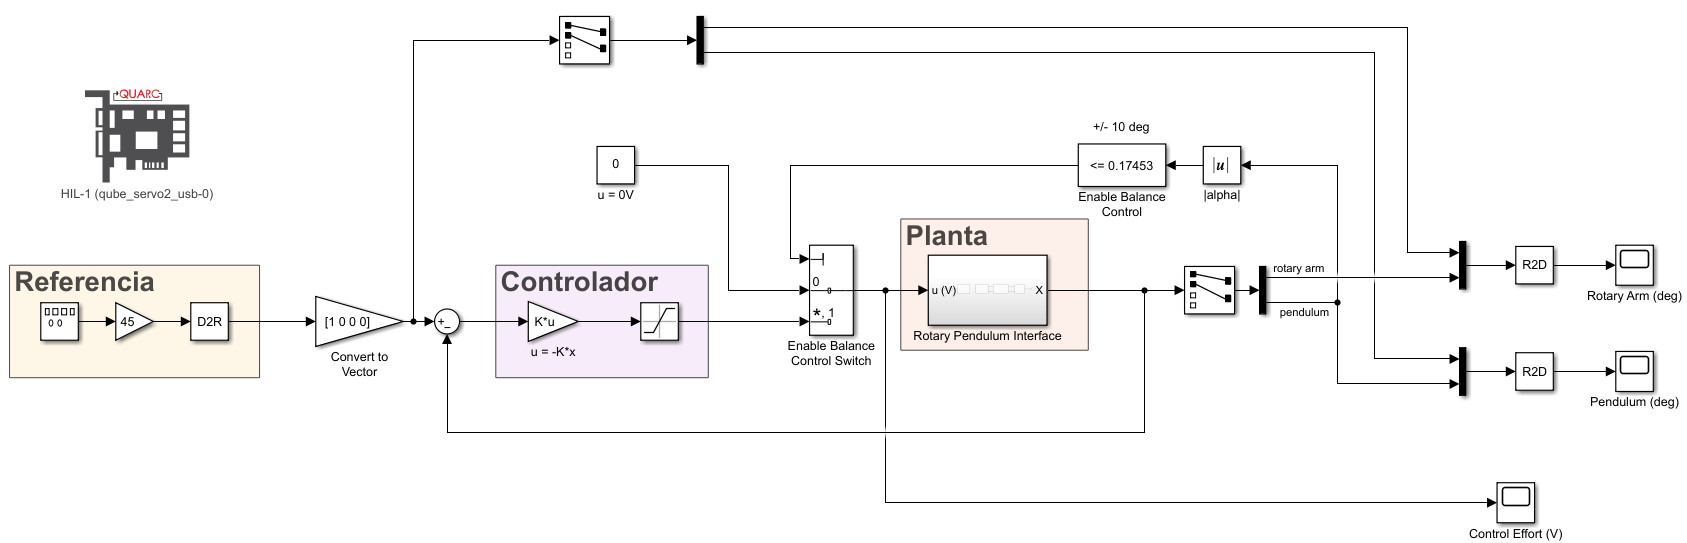
\includegraphics[width=\textwidth]{images/simulink_act2.png}
    \caption{Diagrama de bloques de la Actividad 2 en Simulink.}
    \label{fig:actividad2_diagrama}
\end{figure}








% =============================================================
% CASO 1: Q_mayor y R_opt
% =============================================================
\subsubsection*{Caso 1: $Q_{\text{mayor}}$ y $R_{\text{opt}}$}

Las matrices empleadas para este caso son:
\begin{equation}
Q_{\text{mayor}} = 
\begin{bmatrix}
100 & 0 & 0 & 0 \\
0 & 200 & 0 & 0 \\
0 & 0 & 27 & 0 \\
0 & 0 & 0 & 10
\end{bmatrix}, \qquad 
R_{\text{opt}} = 7
\end{equation}

\begin{equation}
K_1 = \begin{bmatrix} -3.7796 & 83.0938  & -3.3099 &  6.3231\end{bmatrix}
\end{equation}

\begin{figure}[H]
    \centering
    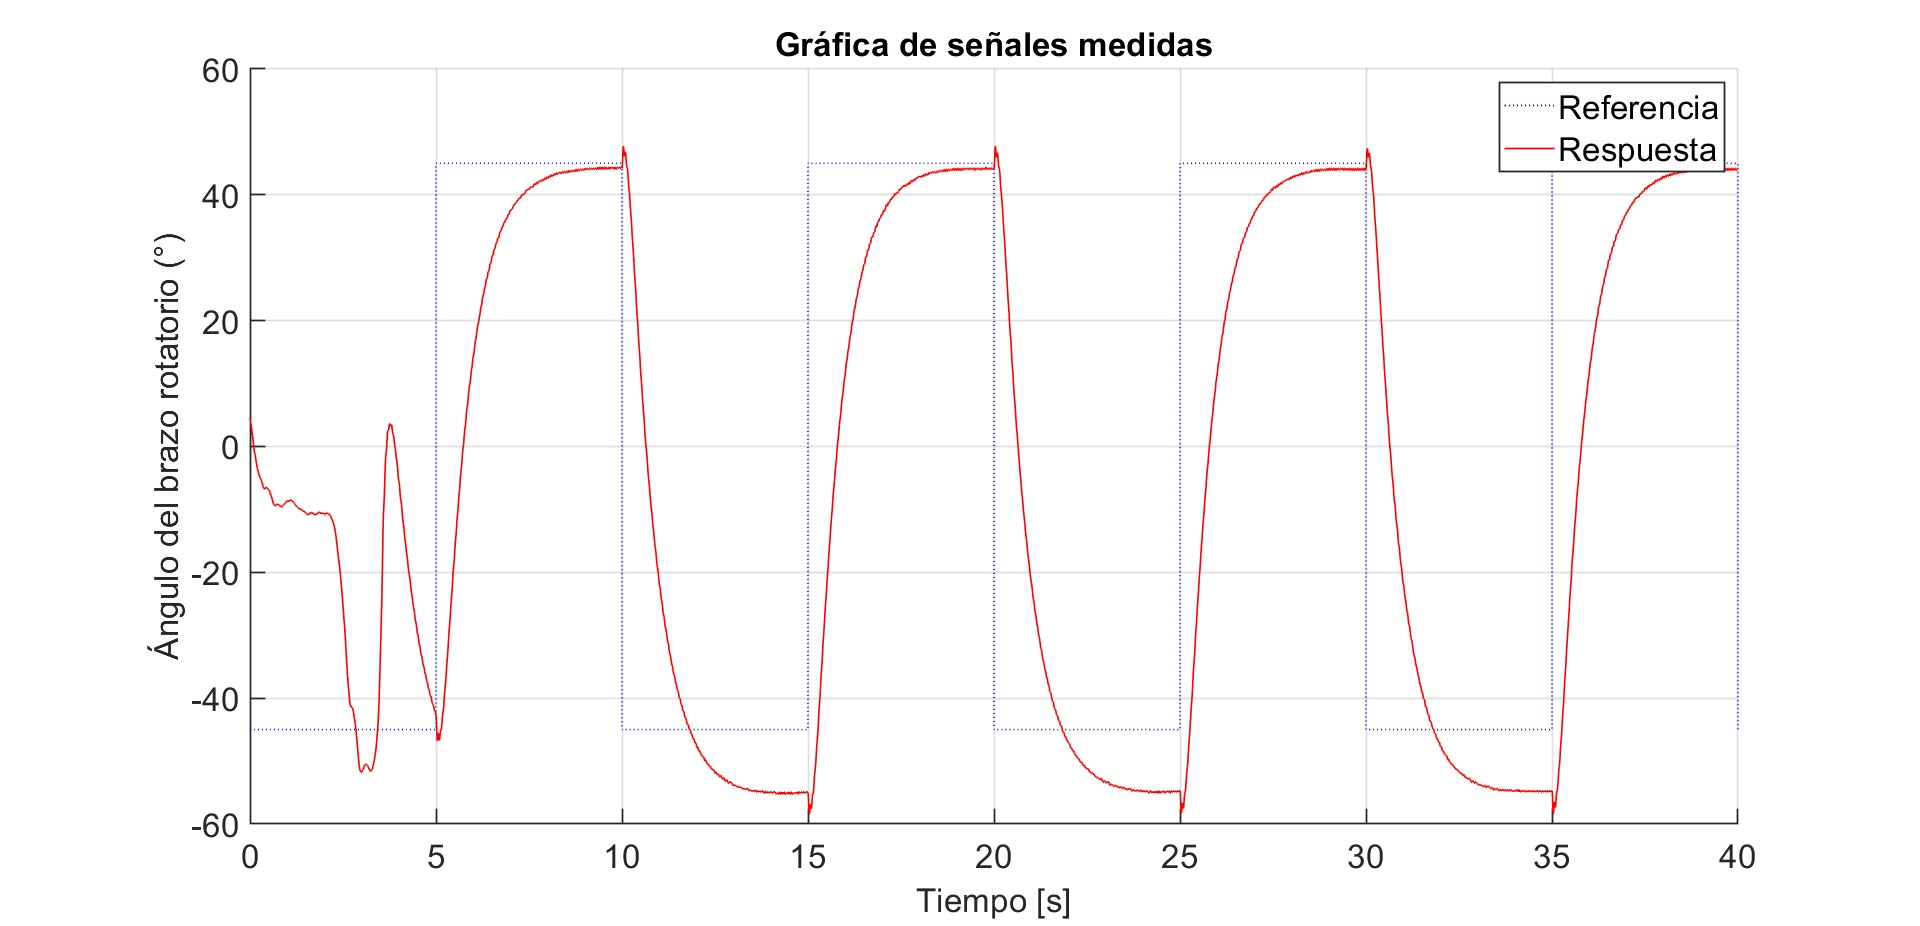
\includegraphics[width=0.85\textwidth]{images/Figura_10.jpg}
    \caption{Caso $Q_{\text{mayor}}$ y $R_{\text{opt}}$: $\theta$ vs. $\theta_{\text{deseado}}$.}
    \label{fig:act2_caso1_theta}
\end{figure}
\noindent Al aumentar $Q_2 = 200$ (peso del péndulo en la función de costo), el controlador prioriza más fuertemente la estabilización del péndulo. Esto reduce el sobreimpulso del brazo a $0.21\%$ (la mitad del caso óptimo) y el tiempo de establecimiento a $2.746$ s. El seguimiento de $\theta_{\text{deseado}}$ es ligeramente más preciso, con un error estacionario de $1.93\%$.
\begin{figure}[H]
    \centering
    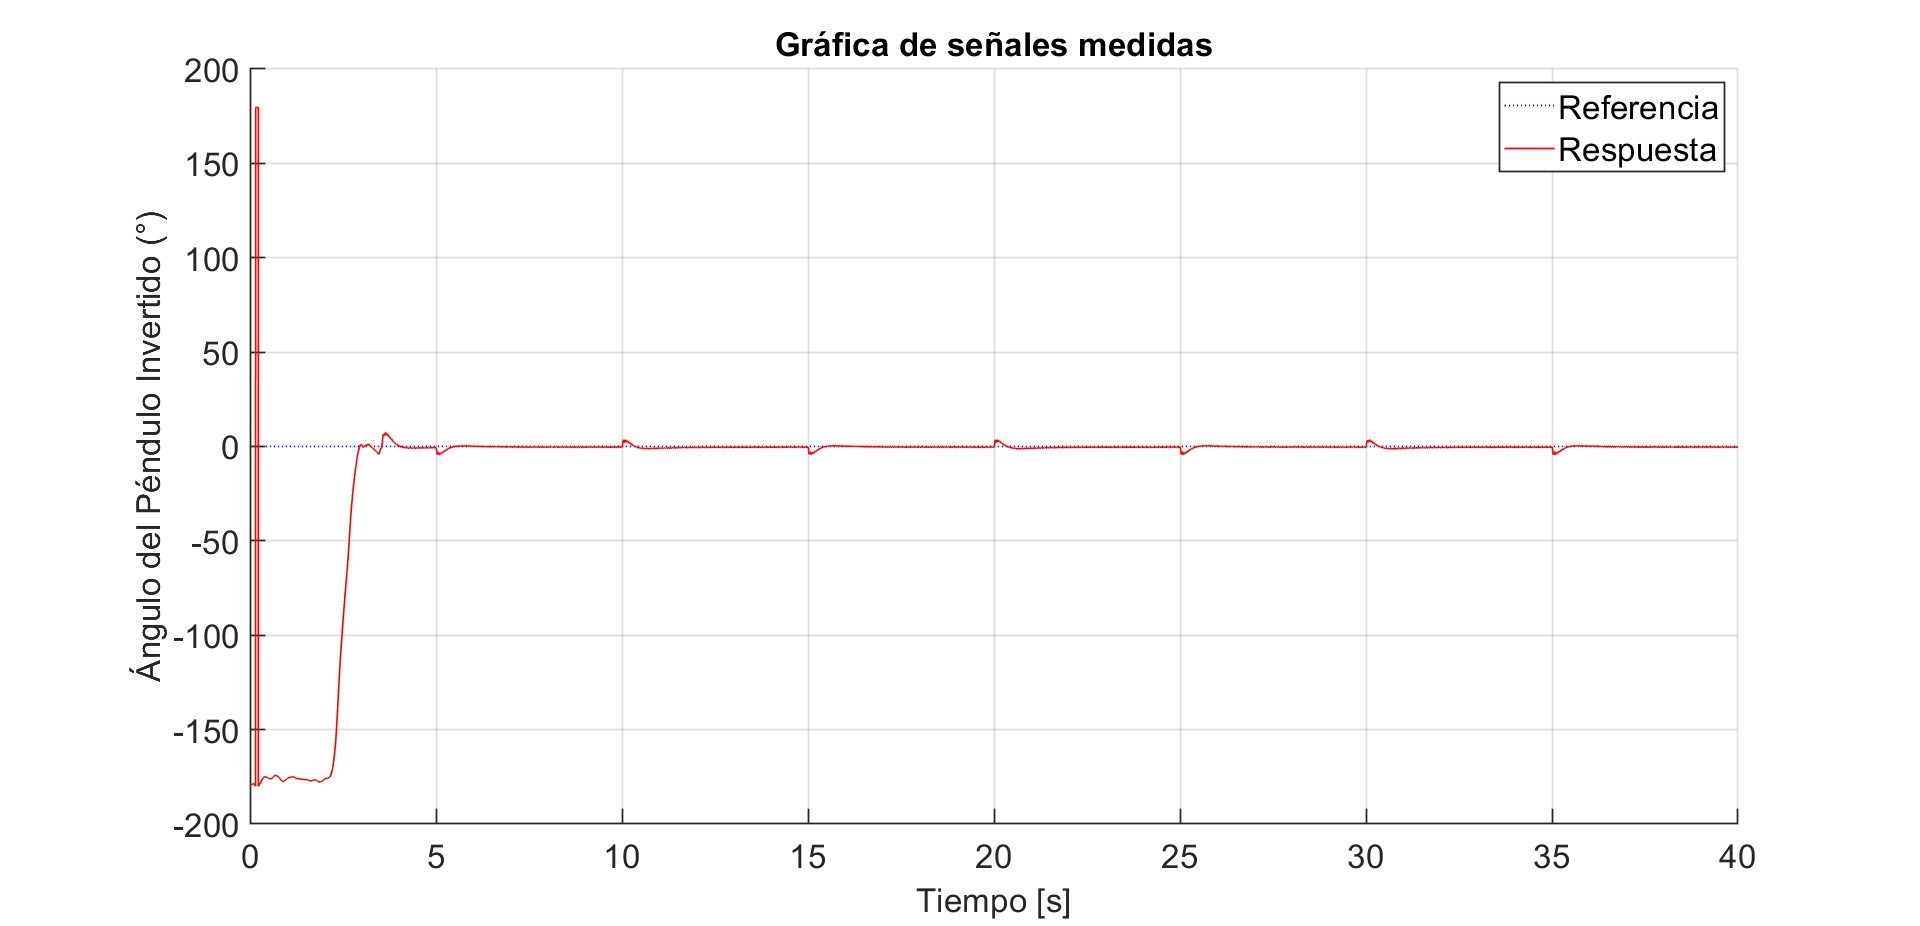
\includegraphics[width=0.85\textwidth]{images/Figura_11.jpg}
    \caption{Caso $Q_{\text{mayor}}$ y $R_{\text{opt}}$: $\alpha$ vs. $\alpha_{\text{deseado}}$.}
    \label{fig:act2_caso1_alpha}
\end{figure}

\begin{figure}[H]
    \centering
    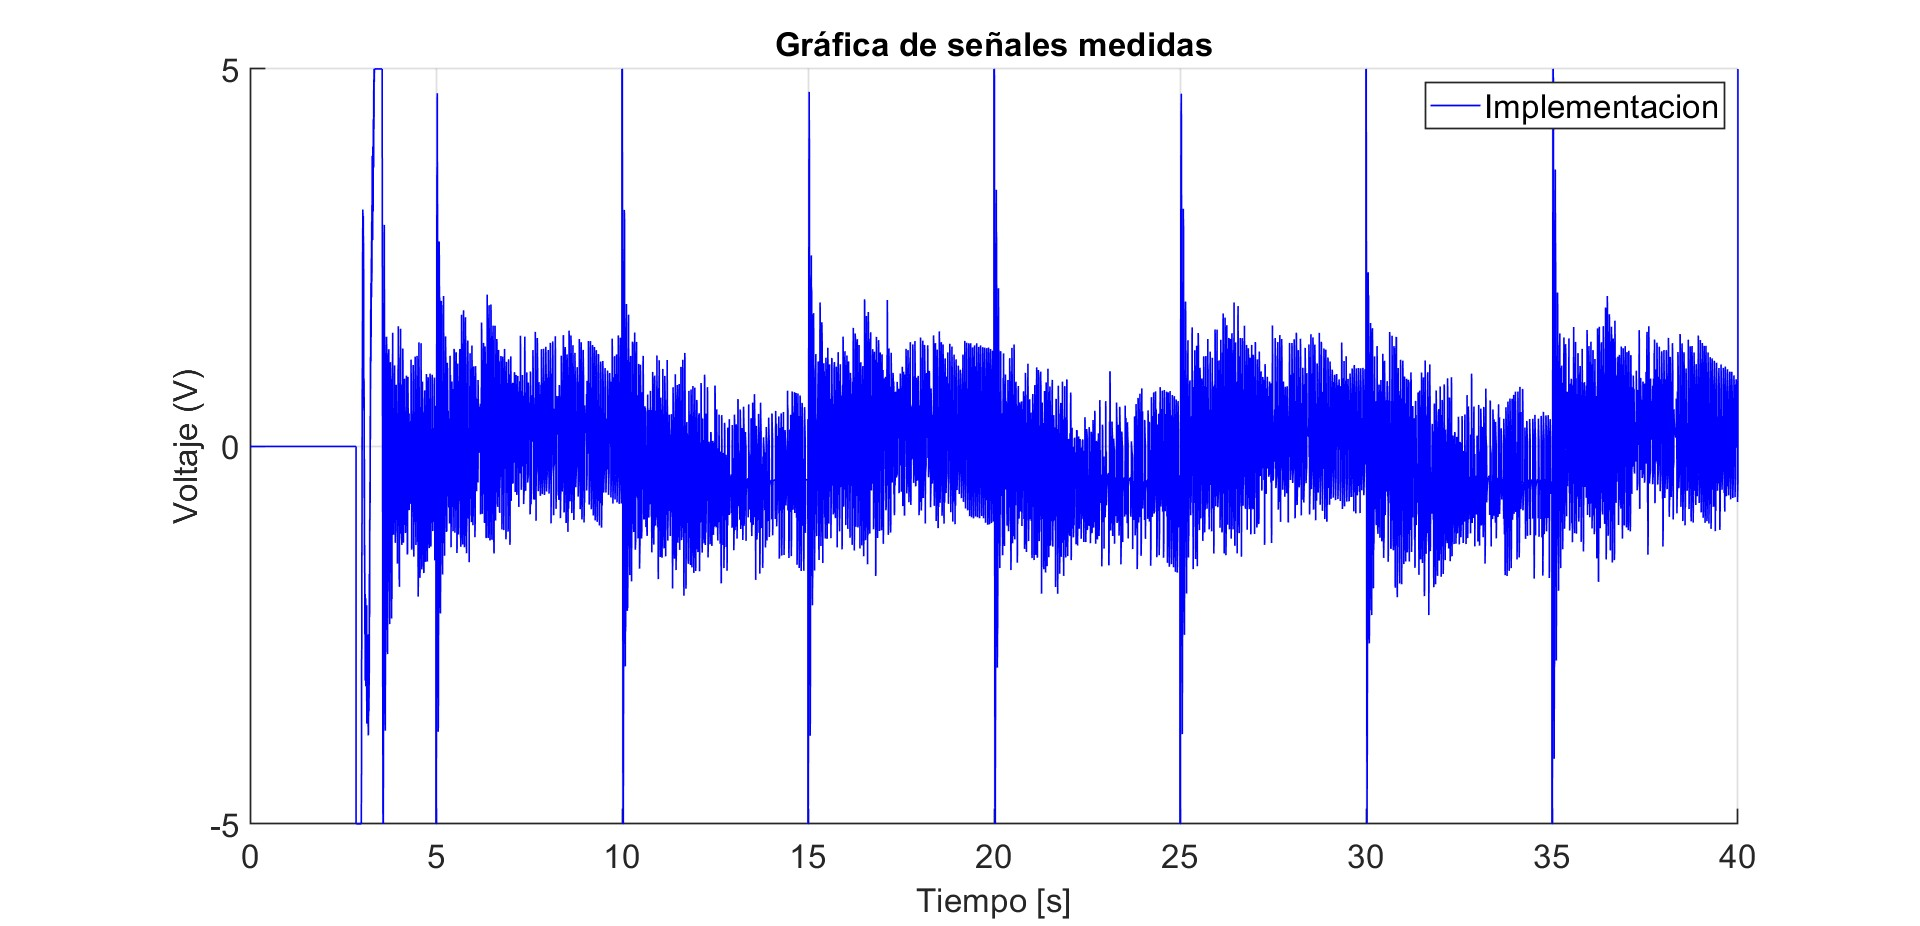
\includegraphics[width=0.85\textwidth]{images/Figura_12.jpg}
    \caption{Caso $Q_{\text{mayor}}$ y $R_{\text{opt}}$: voltaje $V_m$ aplicado al motor.}
    \label{fig:act2_caso1_voltaje}
\end{figure}
\noindent El esfuerzo de control aumenta de manera notable, evidenciando que penalizar más los estados implica un mayor consumo energético del actuador.


% =============================================================
% CASO 2: Q_menor y R_opt
% =============================================================
\subsubsection*{Caso 2: $Q_{\text{menor}}$ y $R_{\text{opt}}$}

Las matrices empleadas para este caso son:

\begin{equation}
Q_{\text{menor}} = 
\begin{bmatrix}
100 & 0 & 0 & 0 \\
0 & 50 & 0 & 0 \\
0 & 0 & 27 & 0 \\
0 & 0 & 0 & 10
\end{bmatrix}, \qquad 
R_{\text{opt}} = 7
\end{equation}

\noindent Vector de ganancias obtenido:
\begin{equation}
K_2 = \begin{bmatrix} -3.7796& 82.8646   & -3.3074  & 6.3172 \end{bmatrix}
\end{equation}

\begin{figure}[H]
    \centering
    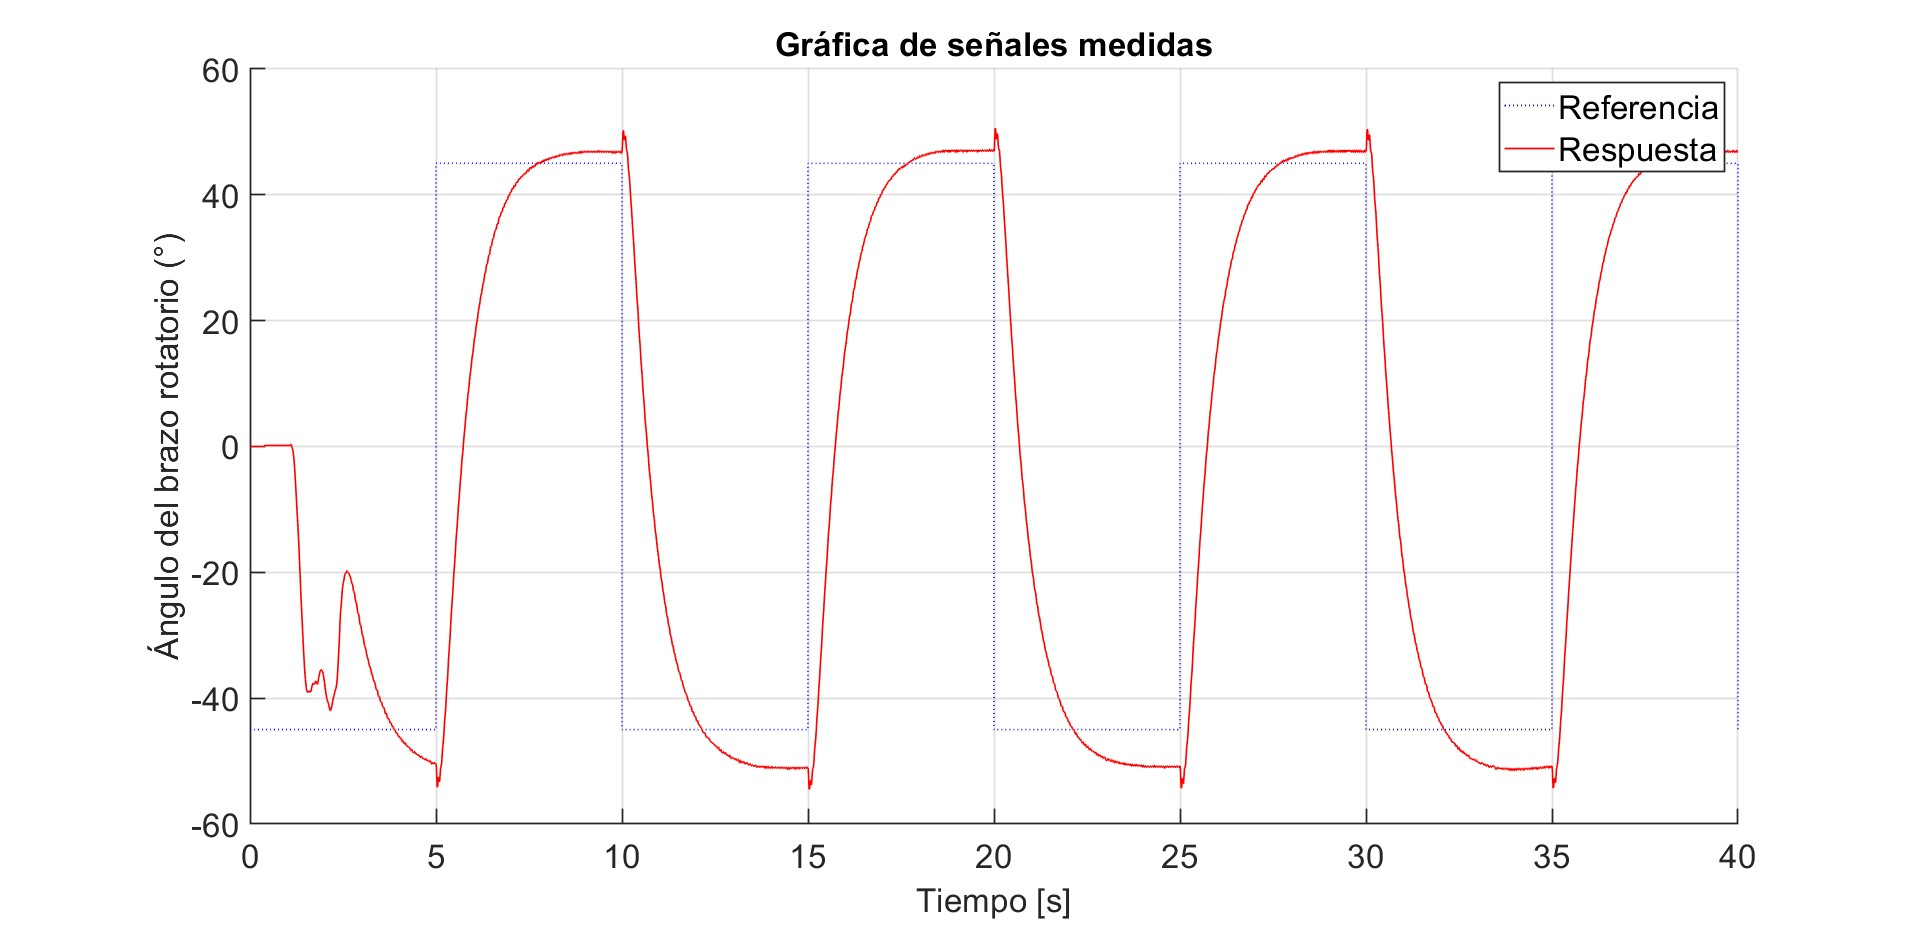
\includegraphics[width=0.85\textwidth]{images/Figura_13.jpg}
    \caption{Caso $Q_{\text{menor}}$ y $R_{\text{opt}}$: $\theta$ vs. $\theta_{\text{deseado}}$.}
    \label{fig:act2_caso2_theta}
\end{figure}
\noindent Al reducir $Q$, el sistema penaliza menos los errores y la respuesta del brazo se vuelve más lenta, con mayor tiempo de establecimiento.

\begin{figure}[H]
    \centering
    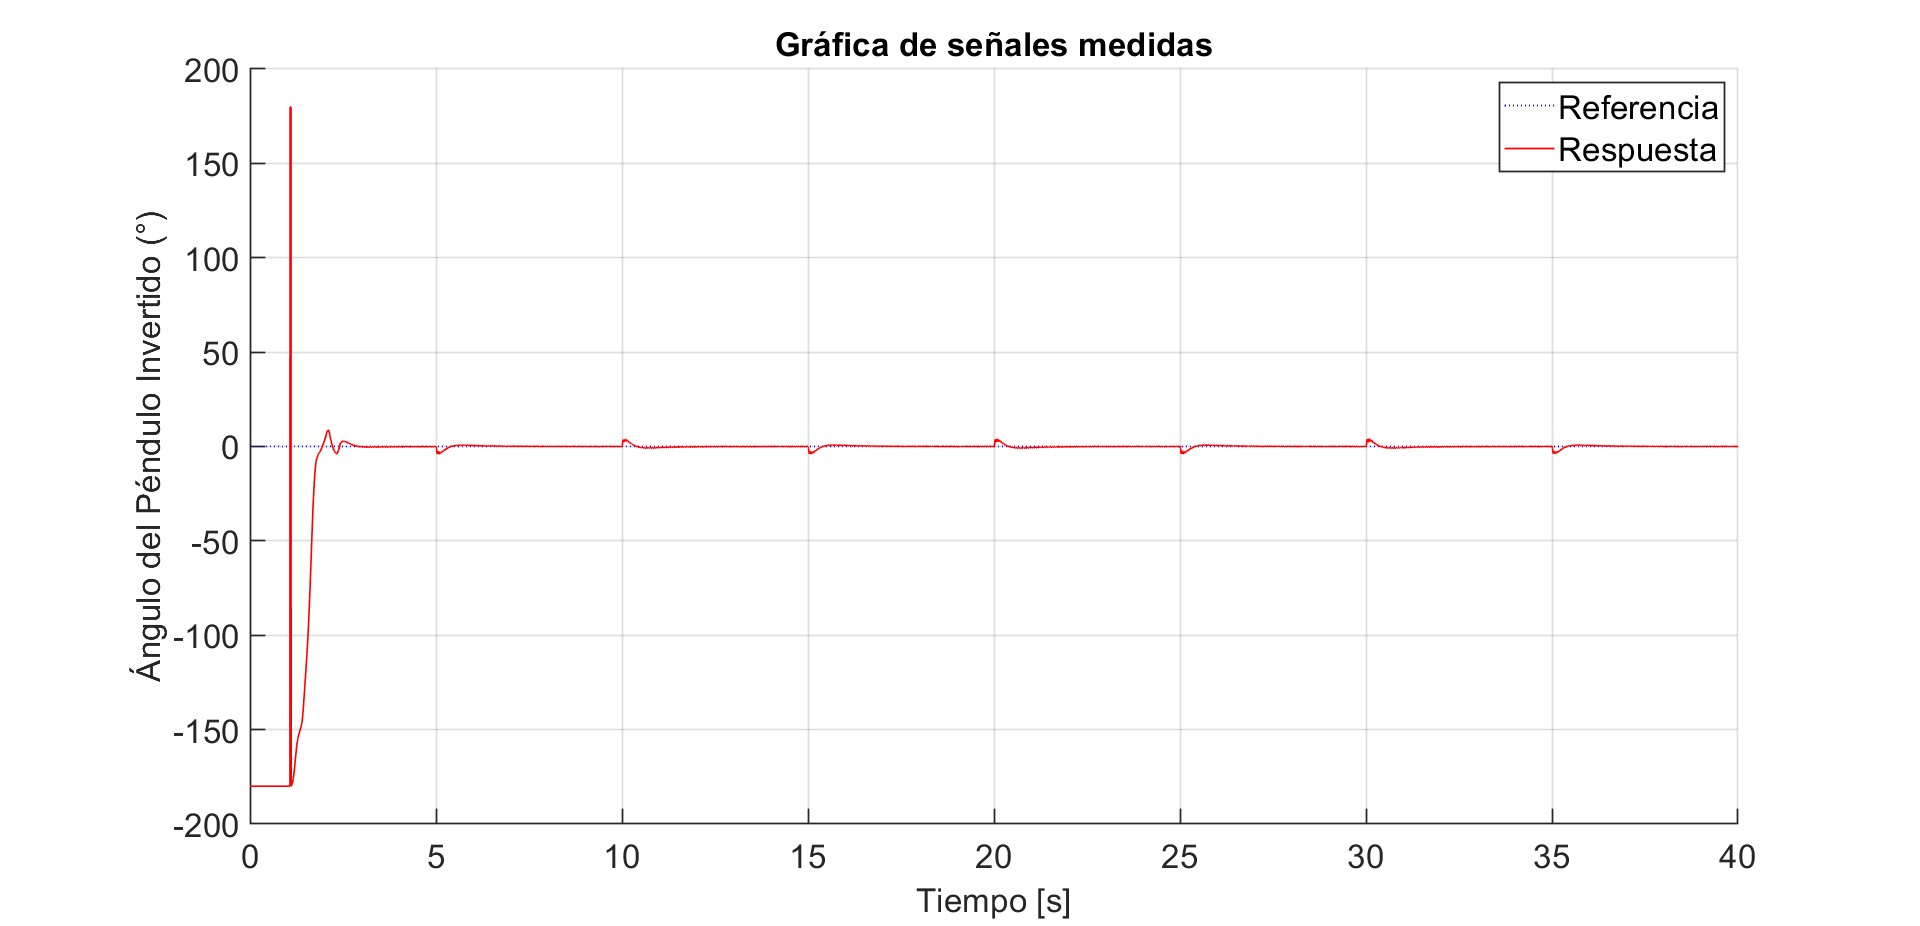
\includegraphics[width=0.85\textwidth]{images/Figura_14.jpg}
    \caption{Caso $Q_{\text{menor}}$ y $R_{\text{opt}}$: $\alpha$ vs. $\alpha_{\text{deseado}}$.}
    \label{fig:act2_caso2_alpha}
\end{figure}
\noindent El péndulo se mantiene cerca de la referencia pero con una corrección más suave, lo que se traduce en una respuesta menos agresiva ante perturbaciones.

\begin{figure}[H]
    \centering
    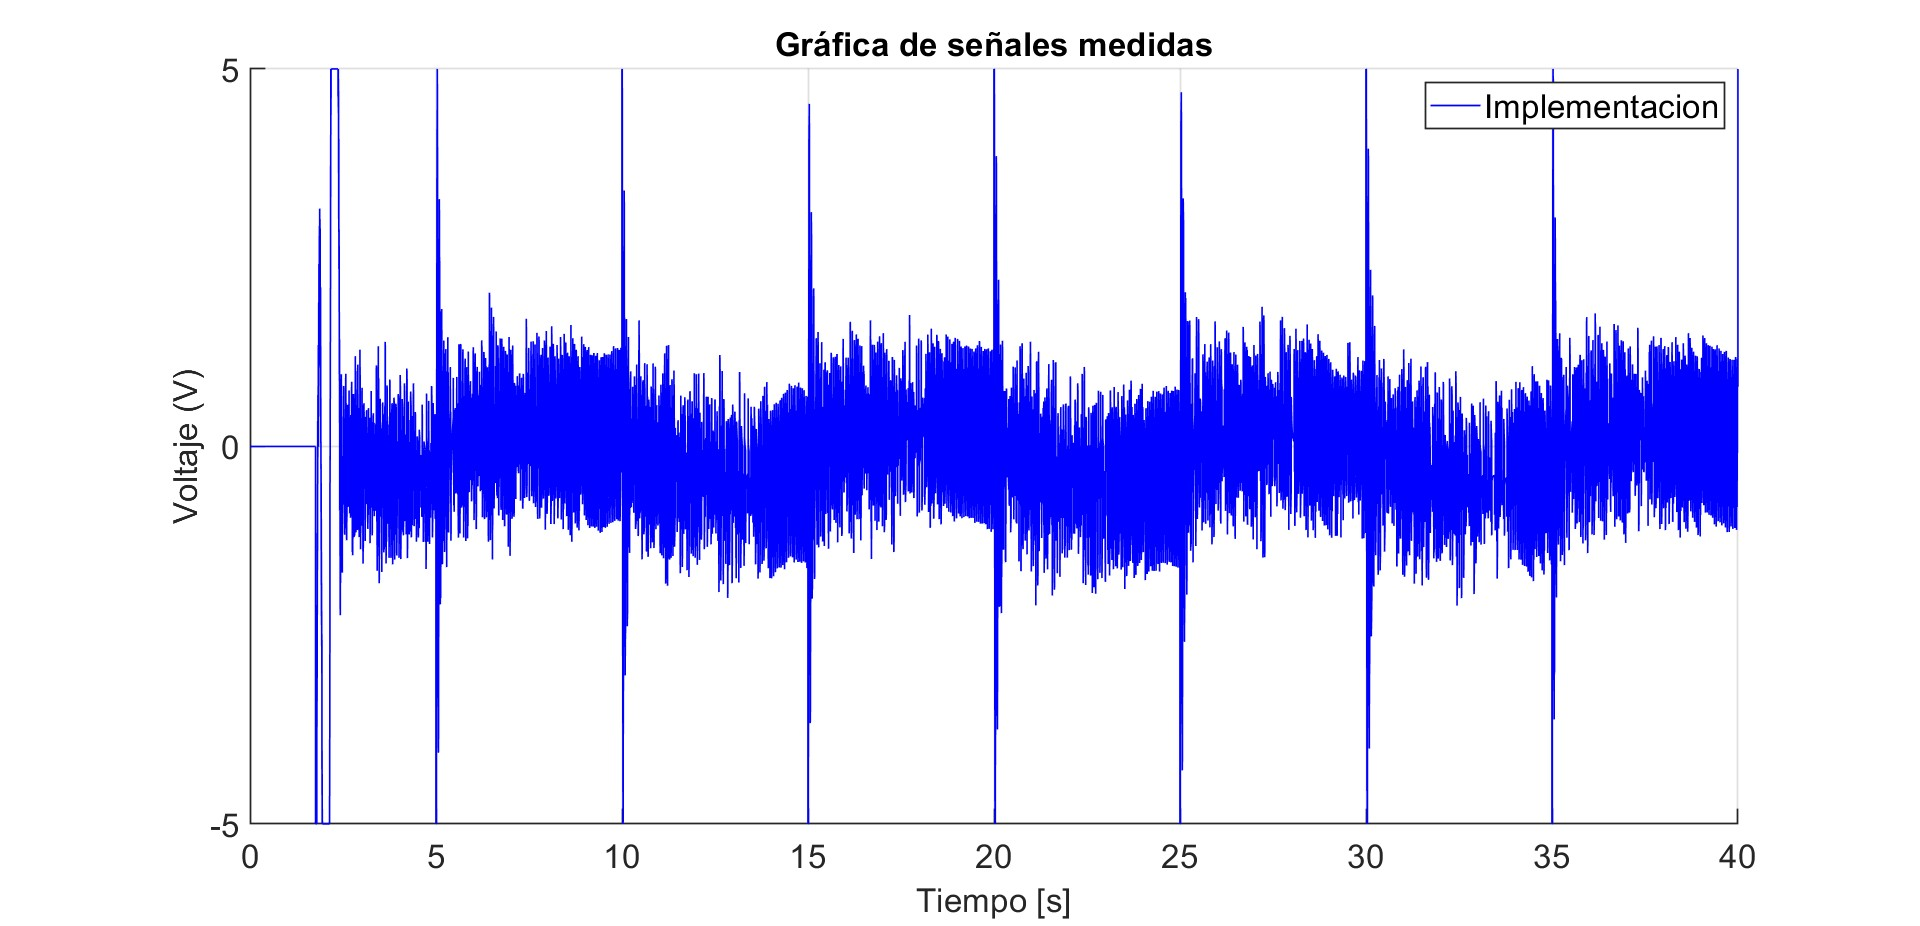
\includegraphics[width=0.85\textwidth]{images/Figura_15.jpg}
    \caption{Caso $Q_{\text{menor}}$ y $R_{\text{opt}}$: voltaje $V_m$ aplicado al motor.}
    \label{fig:act2_caso2_voltaje}
\end{figure}
\noindent El voltaje disminuye respecto al caso óptimo, mostrando que un $Q$ menor reduce el esfuerzo de control a costa de un peor desempeño dinámico.


% =============================================================
% CASO 3: Q_opt y R_mayor
% =============================================================
\subsubsection*{Caso 3: $Q_{\text{opt}}$ y $R_{\text{mayor}}$}

Las matrices empleadas para este caso son:

\begin{equation}
Q_{\text{opt}} = 
\begin{bmatrix}
100 & 0 & 0 & 0 \\
0 & 100 & 0 & 0 \\
0 & 0 & 27 & 0 \\
0 & 0 & 0 & 10
\end{bmatrix}, \qquad 
R_{\text{mayor}} = 10
\end{equation}

\noindent Vector de ganancias obtenido:

\begin{equation}
K_3 = \begin{bmatrix} -3.1623 &   72.7865 &   -2.8514   &  5.4981 \end{bmatrix}
\end{equation}

\begin{figure}[H]
    \centering
    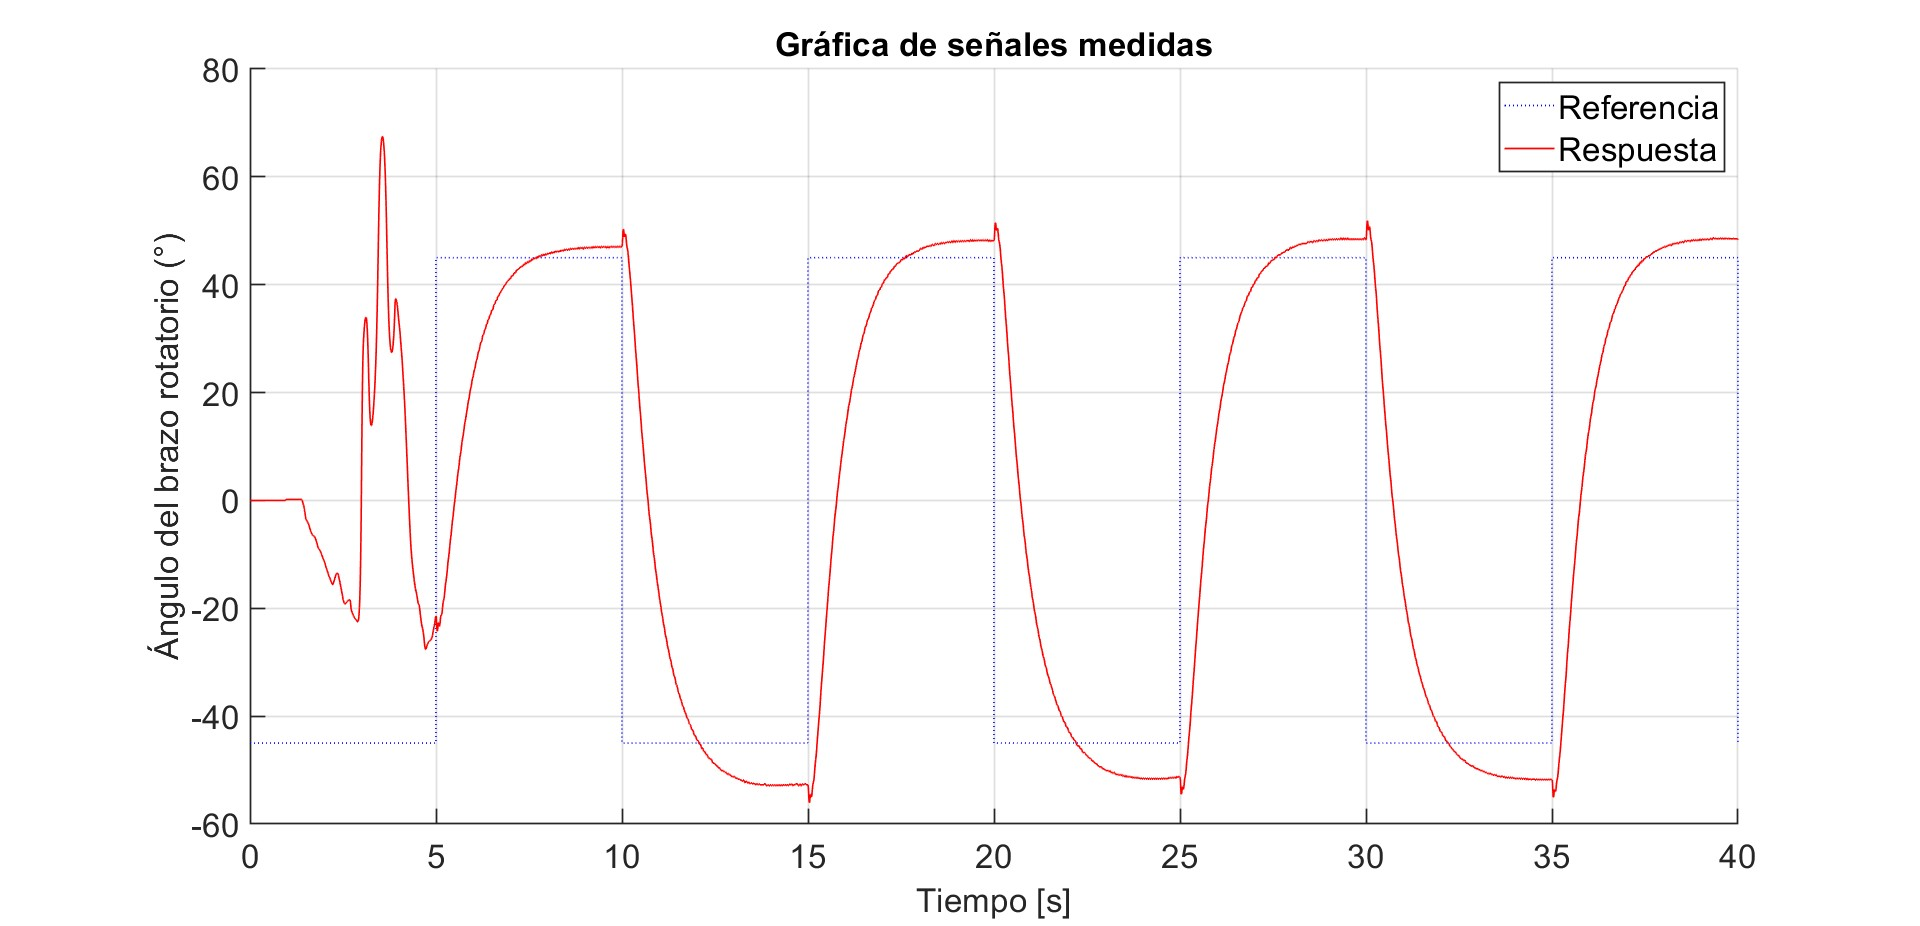
\includegraphics[width=0.85\textwidth]{images/Figura_16.jpg}
    \caption{Caso $Q_{\text{opt}}$ y $R_{\text{mayor}}$: $\theta$ vs. $\theta_{\text{deseado}}$.}
    \label{fig:act2_caso3_theta}
\end{figure}
\noindent Aumentar $R$ implica penalizar más el esfuerzo de control, por lo que la respuesta del brazo se vuelve más lenta y conservadora.

\begin{figure}[H]
    \centering
    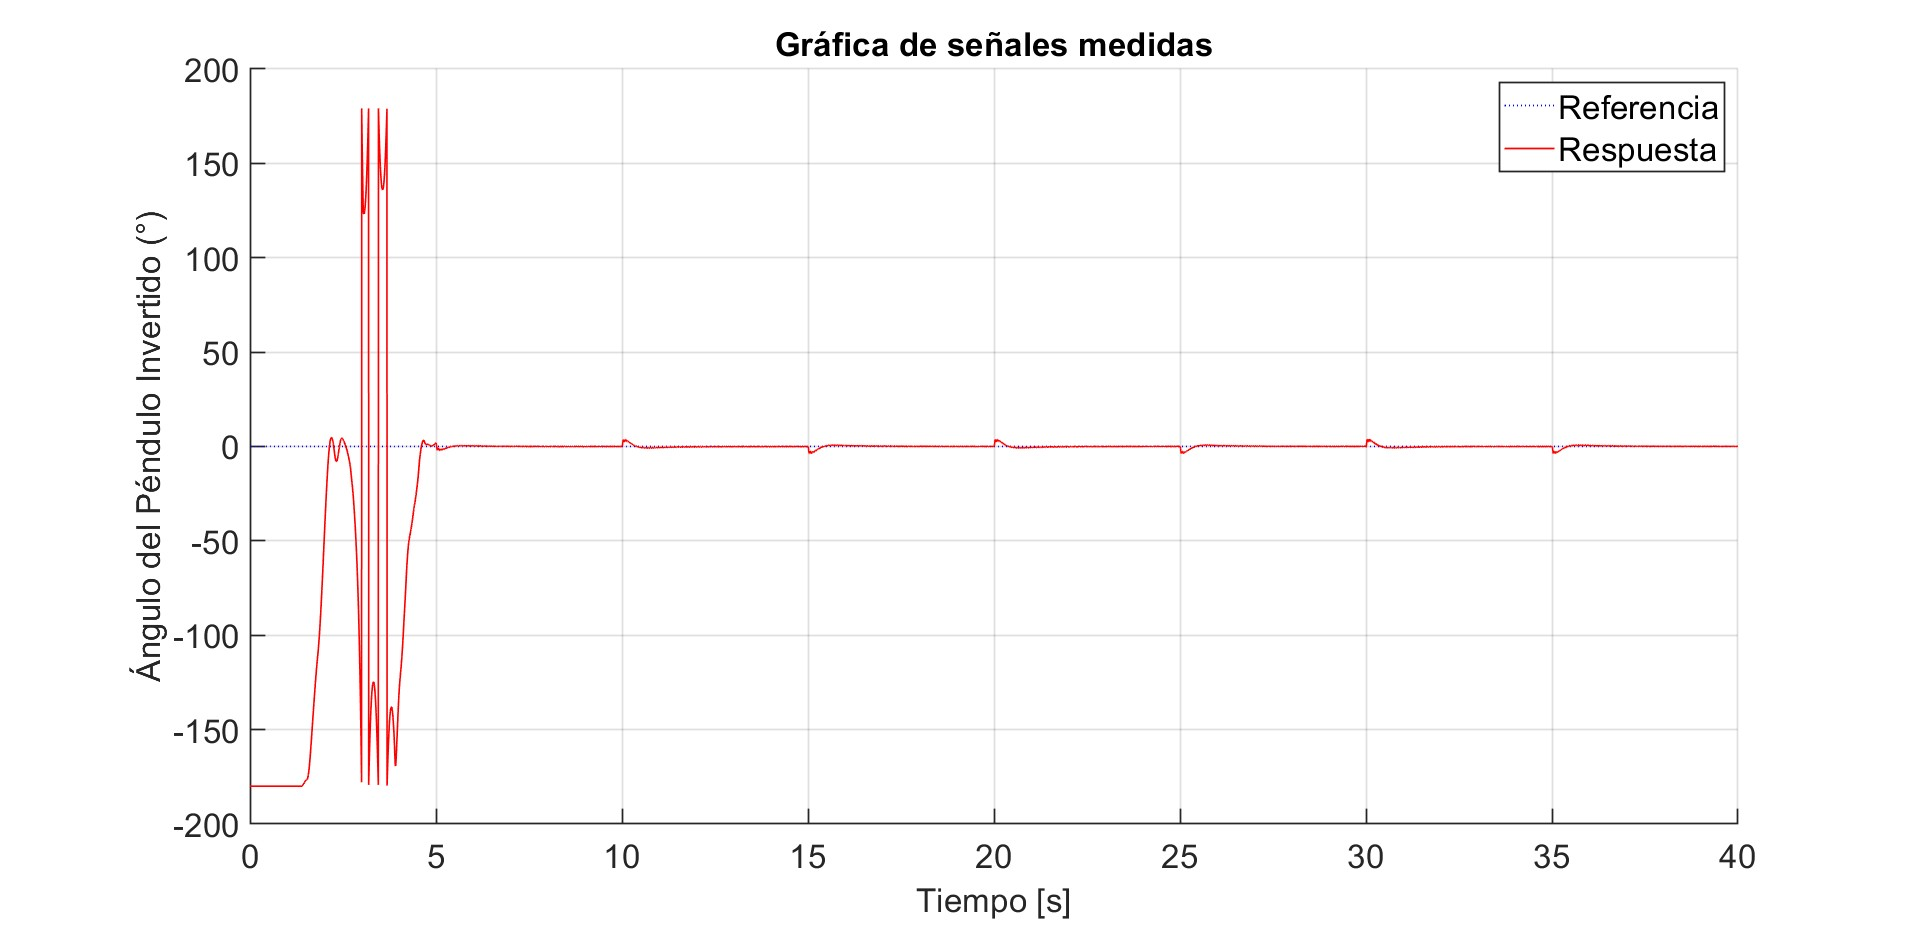
\includegraphics[width=0.85\textwidth]{images/Figura_17.jpg}
    \caption{Caso $Q_{\text{opt}}$ y $R_{\text{mayor}}$: $\alpha$ vs. $\alpha_{\text{deseado}}$.}
    \label{fig:act2_caso3_alpha}
\end{figure}
\noindent El péndulo tarda más en estabilizarse en la posición invertida, ya que el controlador prioriza ahorrar energía sobre corregir rápidamente los errores.

\begin{figure}[H]
    \centering
    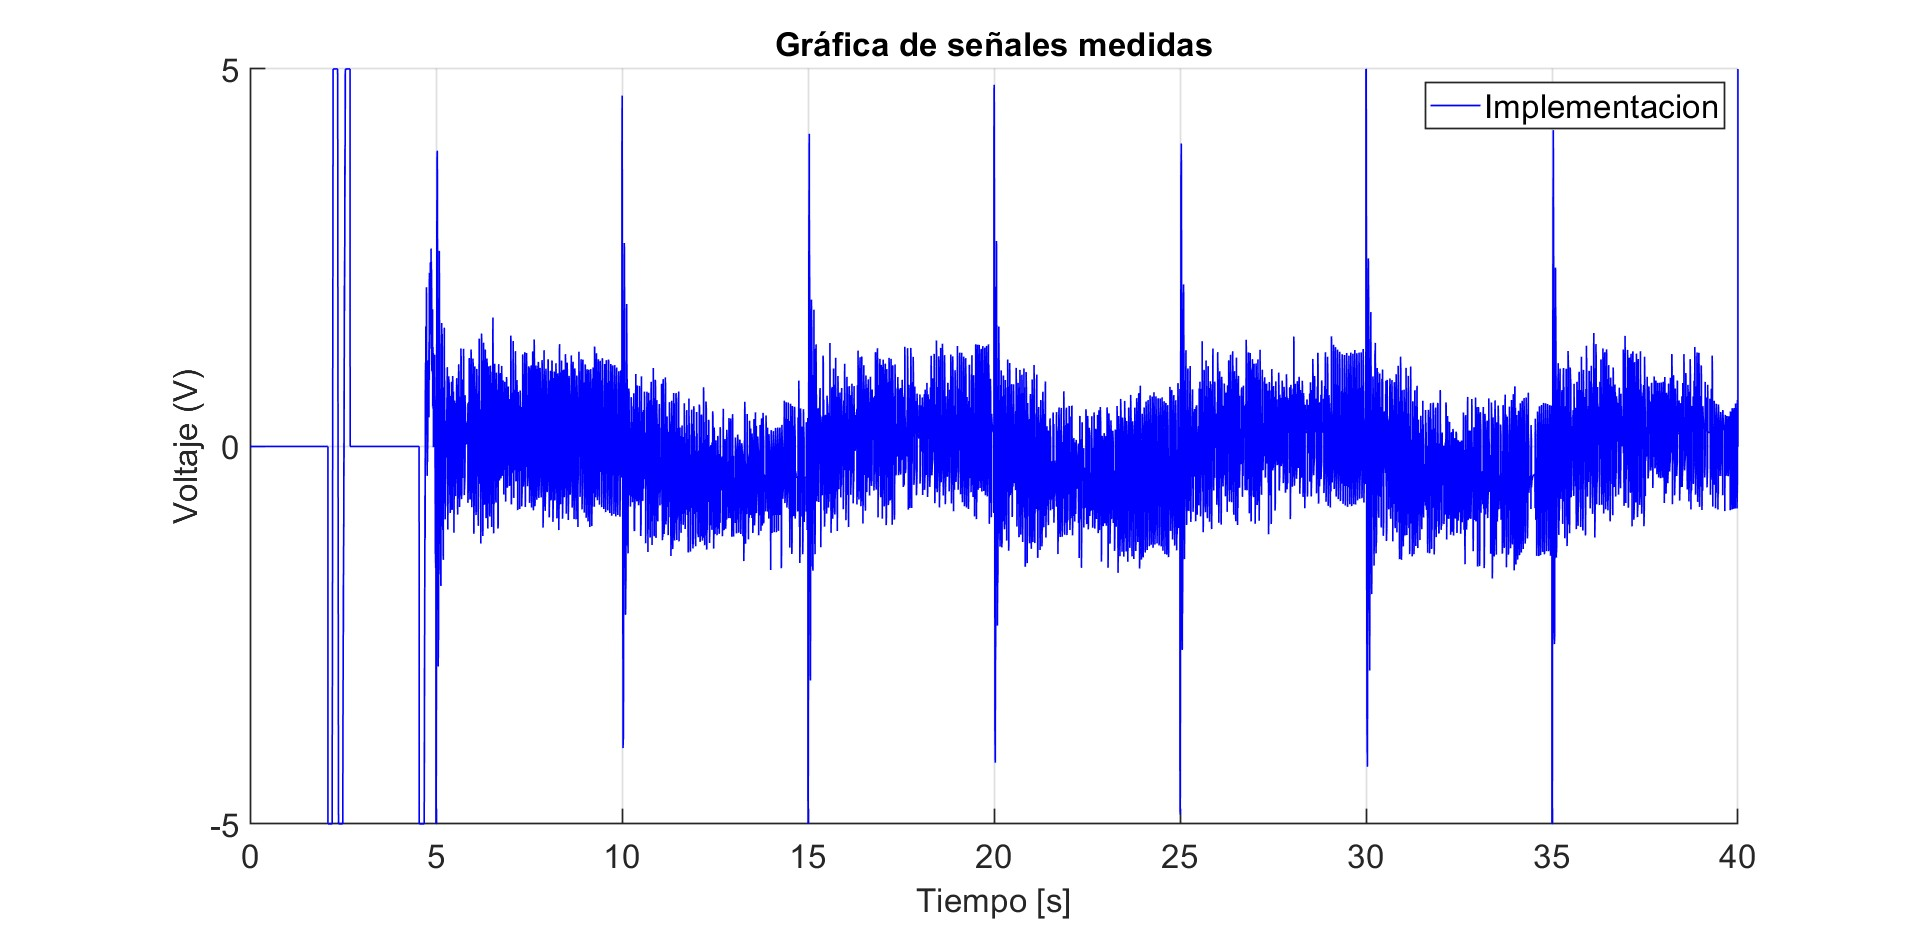
\includegraphics[width=0.85\textwidth]{images/Figura_18.jpg}
    \caption{Caso $Q_{\text{opt}}$ y $R_{\text{mayor}}$: voltaje $V_m$ aplicado al motor.}
    \label{fig:act2_caso3_voltaje}
\end{figure}
\noindent El voltaje aplicado es claramente más bajo, evidenciando que un $R$ mayor reduce el esfuerzo de control a costa de un desempeño más lento.


% =============================================================
% CASO 4: Q_opt y R_menor
% =============================================================
\subsubsection*{Caso 4: $Q_{\text{opt}}$ y $R_{\text{menor}}$}

Las matrices empleadas para este caso son:

\begin{equation}
Q_{\text{opt}} = 
\begin{bmatrix}
100 & 0 & 0 & 0 \\
0 & 100 & 0 & 0 \\
0 & 0 & 27 & 0 \\
0 & 0 & 0 & 10
\end{bmatrix}, \qquad 
R_{\text{menor}} = 4
\end{equation}

\noindent Vector de ganancias obtenido:

\begin{equation}
K_4 = \begin{bmatrix}    -5.0000  & 103.1951   & -4.2155     &7.9584 \end{bmatrix}
\end{equation}

\begin{figure}[H]
    \centering
    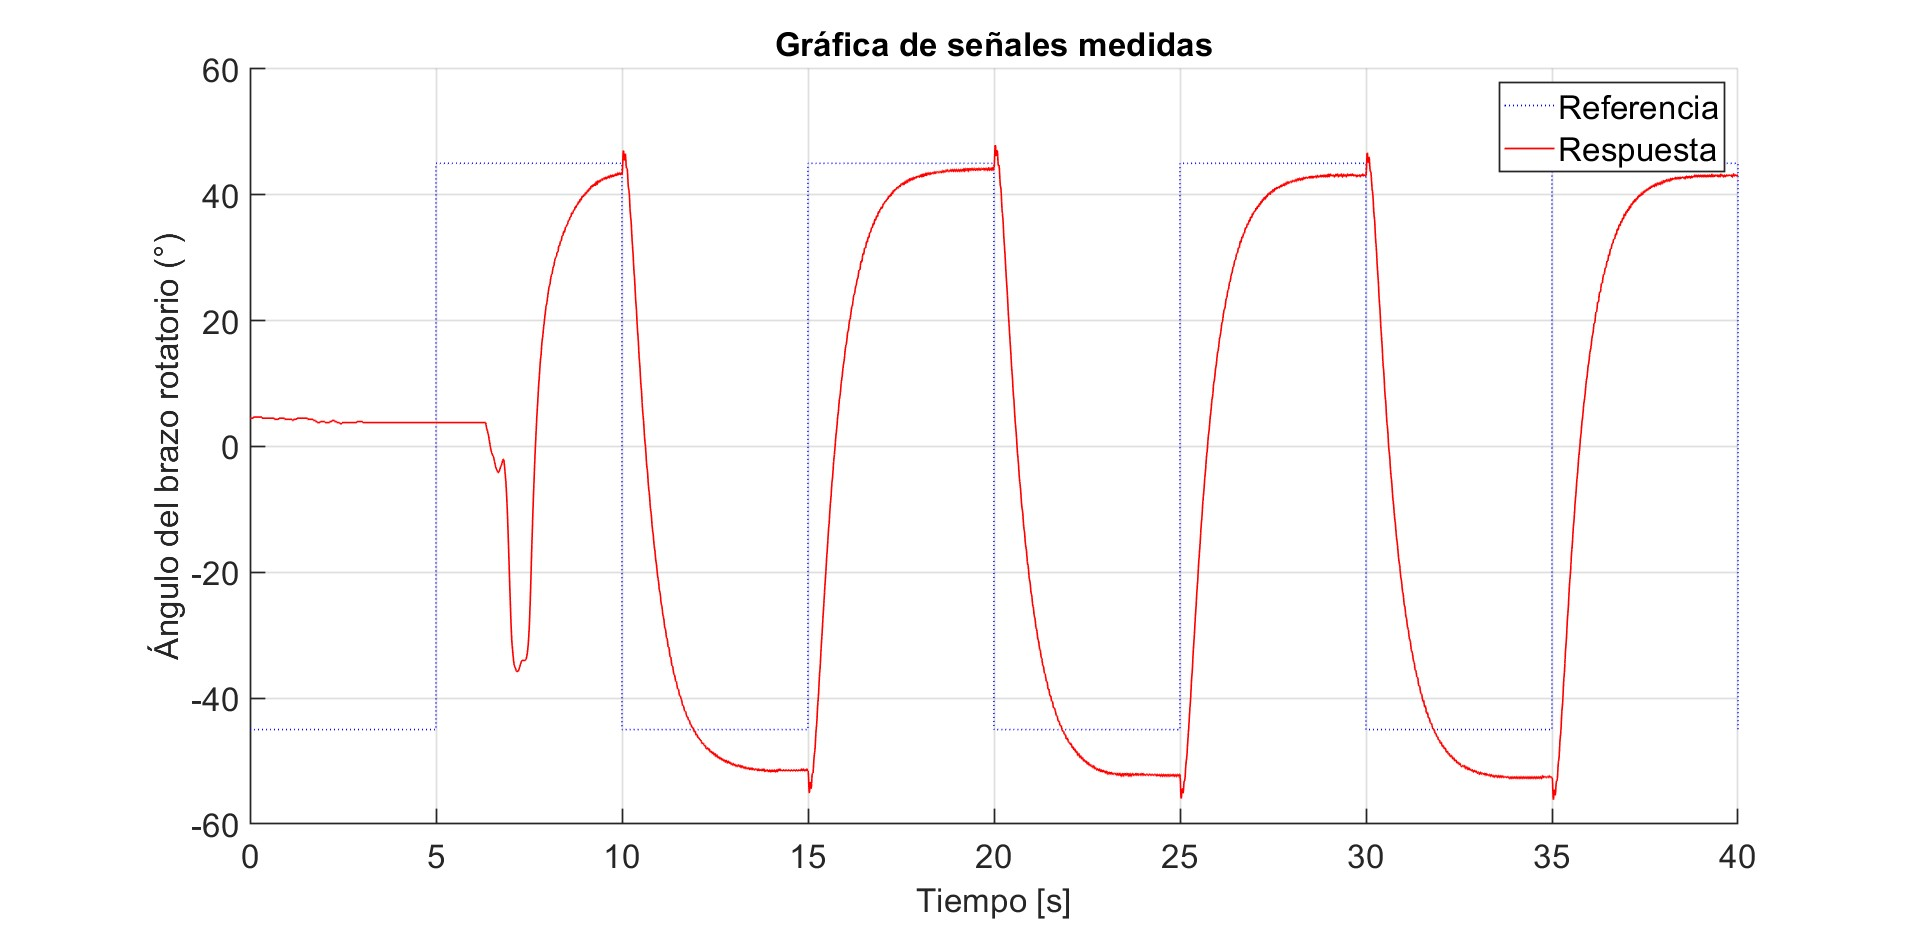
\includegraphics[width=0.85\textwidth]{images/Figura_19.jpg}
    \caption{Caso $Q_{\text{opt}}$ y $R_{\text{menor}}$: $\theta$ vs. $\theta_{\text{deseado}}$.}
    \label{fig:act2_caso4_theta}
\end{figure}
\noindent Reducir $R$ libera al controlador para usar más esfuerzo, por lo que la respuesta del brazo es más rápida y agresiva.

\begin{figure}[H]
    \centering
    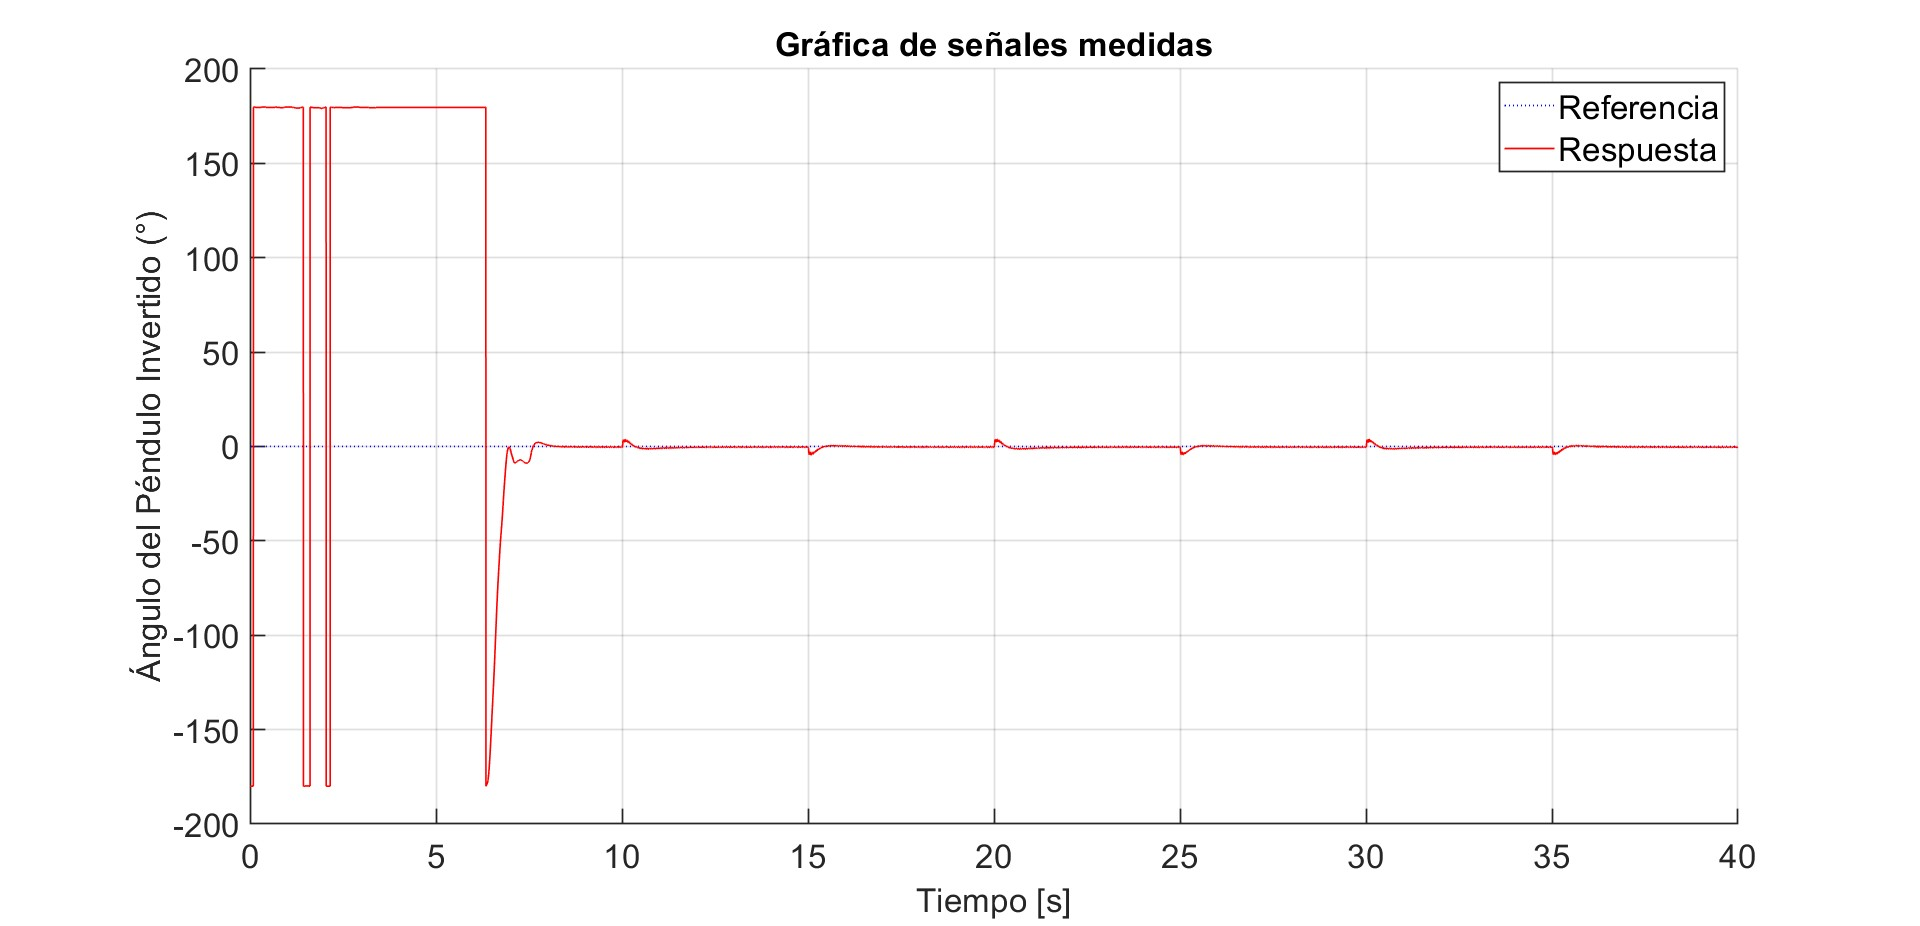
\includegraphics[width=0.85\textwidth]{images/Figura_20.jpg}
    \caption{Caso $Q_{\text{opt}}$ y $R_{\text{menor}}$: $\alpha$ vs. $\alpha_{\text{deseado}}$.}
    \label{fig:act2_caso4_alpha}
\end{figure}
\noindent El péndulo se mantiene más cerca de la referencia con correcciones rápidas, aunque la actividad del controlador puede generar oscilaciones de mayor frecuencia.

\begin{figure}[H]
    \centering
    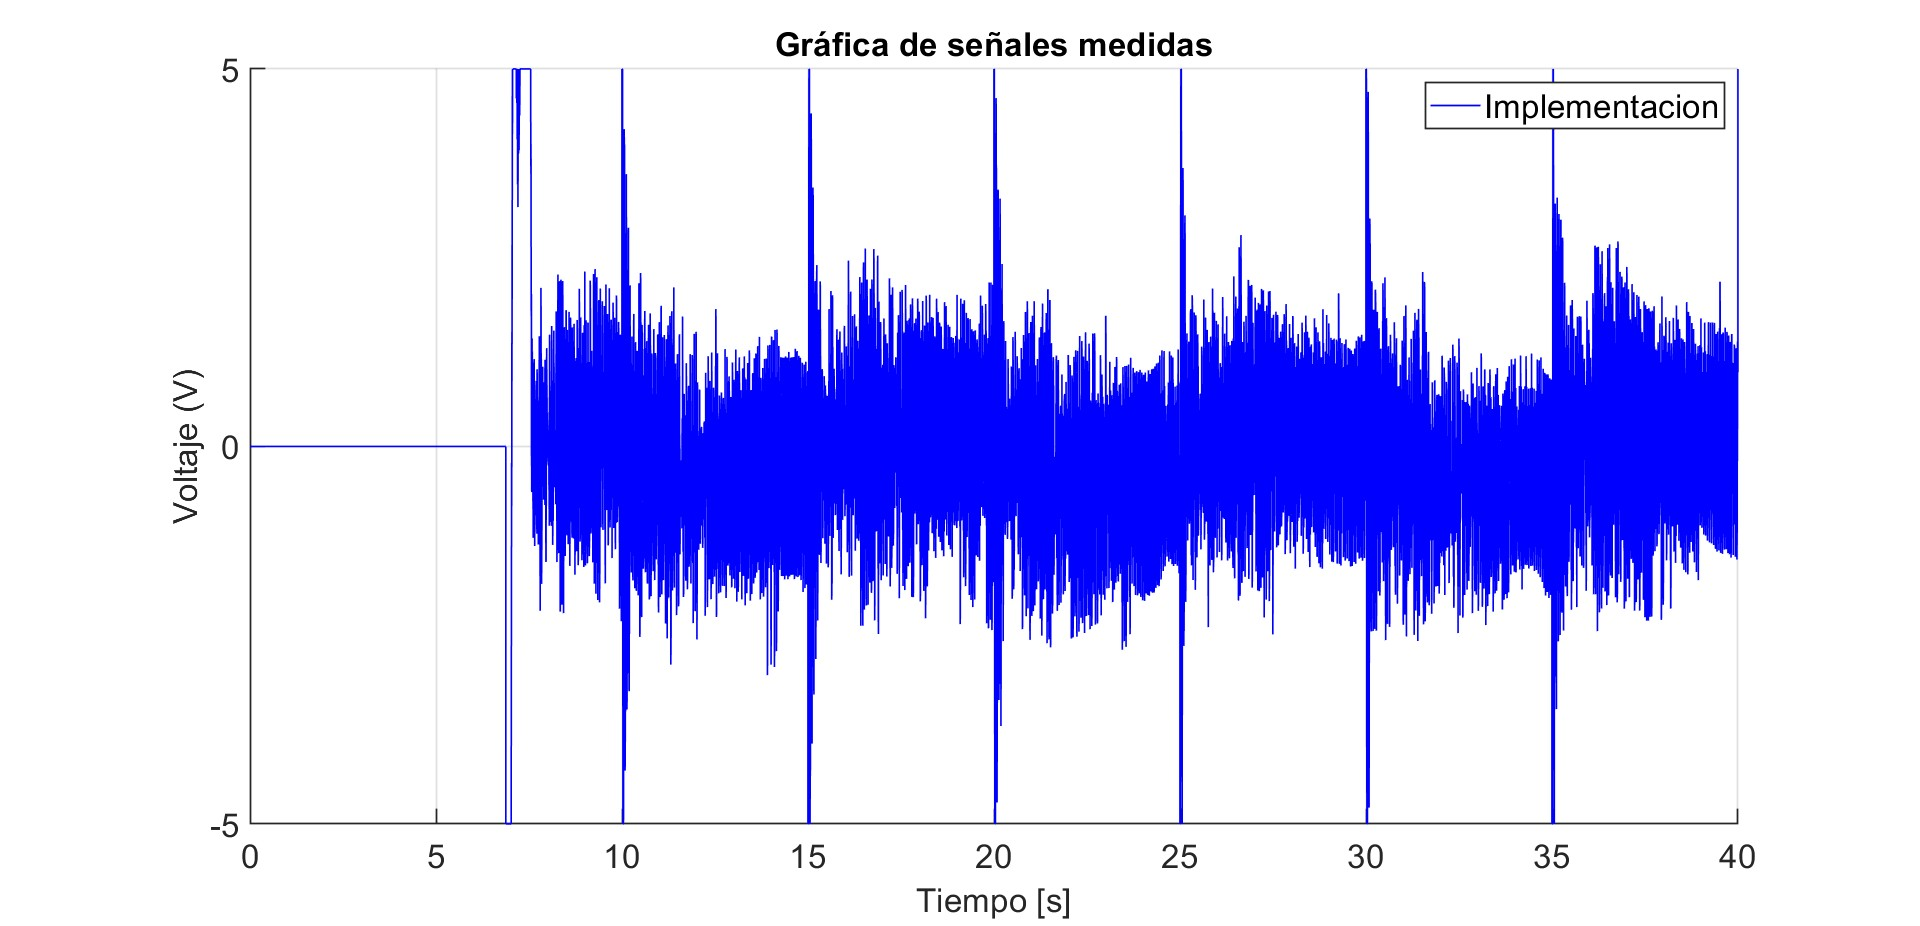
\includegraphics[width=0.85\textwidth]{images/Figura_21.jpg}
    \caption{Caso $Q_{\text{opt}}$ y $R_{\text{menor}}$: voltaje $V_m$ aplicado al motor.}
    \label{fig:act2_caso4_voltaje}
\end{figure}
\noindent El voltaje aplicado aumenta de manera significativa, reflejando que un $R$ menor permite mayor esfuerzo de control y, por ende, mayor consumo del actuador.


% =============================================================
% CUADRO COMPARATIVO ACTIVIDAD 2
% =============================================================
\subsubsection*{Cuadro comparativo}

Presente un cuadro comparativo que permita discutir cómo afecta aumentar o disminuir \textbf{Q} y \textbf{R} sobre la respuesta del sistema y el esfuerzo de control.

\begin{table}[H]
\centering
\caption{Comparación de parámetros de desempeño del control de $\theta$ al variar $Q$ y $R$.}
\label{tab:act2_comparativo}
\renewcommand{\arraystretch}{1.3}
\begin{tabular}{|c|c|c|c|}
\hline
\textbf{Caso} & \textbf{Sobreimpulso (\%)} & \textbf{$t_s$ (s)} & \textbf{$e_{ss}$ (\%)} \\\hline
$Q_{\text{opt}}$, $R_{\text{opt}}$      & $0.42$ & $2.926$ & $2.10$ \\\hline
$Q_{\text{mayor}}$, $R_{\text{opt}}$    & $0.21$ & $2.746$ & $1.93$ \\\hline
$Q_{\text{menor}}$, $R_{\text{opt}}$    & $0.17$ & $2.614$ & $4.51$ \\\hline
$Q_{\text{opt}}$, $R_{\text{mayor}}$    & $0.26$ & $2.832$ & $7.14$ \\\hline
$Q_{\text{opt}}$, $R_{\text{menor}}$    & $0.33$ & $2.626$ & $2.04$ \\\hline
\end{tabular}
\end{table}

\noindent A partir de la Tabla~\ref{tab:act2_comparativo} se observa lo siguiente: aumentar $Q_2$ (de $100$ a $200$) reduce el sobreimpulso y el error estacionario, manteniendo un tiempo de establecimiento similar, lo cual indica una respuesta más precisa a costa de mayor esfuerzo de control. Por el contrario, disminuir $Q_2$ (de $100$ a $50$) reduce ligeramente el sobreimpulso pero \textbf{deteriora notablemente el error estacionario} ($4.51\%$), evidenciando una respuesta menos precisa. En cuanto a $R$: aumentar $R$ (de $7$ a $10$) produce el peor error estacionario ($7.14\%$), confirmando que penalizar más el esfuerzo de control reduce la capacidad de seguimiento de la referencia; mientras que disminuir $R$ (de $7$ a $4$) mejora ligeramente el error estacionario y reduce el tiempo de establecimiento, a costa de mayor consumo de voltaje. El caso óptimo $(Q_{\text{opt}}, R_{\text{opt}})$ representa un equilibrio adecuado entre todos los parámetros, cumpliendo las especificaciones de desempeño.
\noindent Del cuadro comparativo se concluye que aumentar $Q$ o disminuir $R$ produce una respuesta más rápida pero con mayor esfuerzo de control y oscilaciones más marcadas, mientras que disminuir $Q$ o aumentar $R$ genera una respuesta más conservadora con menor consumo de energía pero mayor tiempo de establecimiento. El caso óptimo corresponde al equilibrio entre desempeño dinámico y esfuerzo de control.


\subsection*{Actividad 3. Análisis del algoritmo swing-up}
Utilice el archivo de Simulink \texttt{act3\_q\_qube\_swing\_up.slx} y emplee el vector de ganancias \textbf{K} obtenido a partir de los valores óptimos $Q_{\text{opt}}$ y $R_{\text{opt}}$ determinados en la \textbf{Actividad 1}. Utilice un tiempo de implementación de \textbf{20s}. En esta actividad deberá explicar paso a paso cómo funciona el algoritmo \textbf{swing-up} del diagrama de bloques.
\begin{figure}[H]
    \centering
    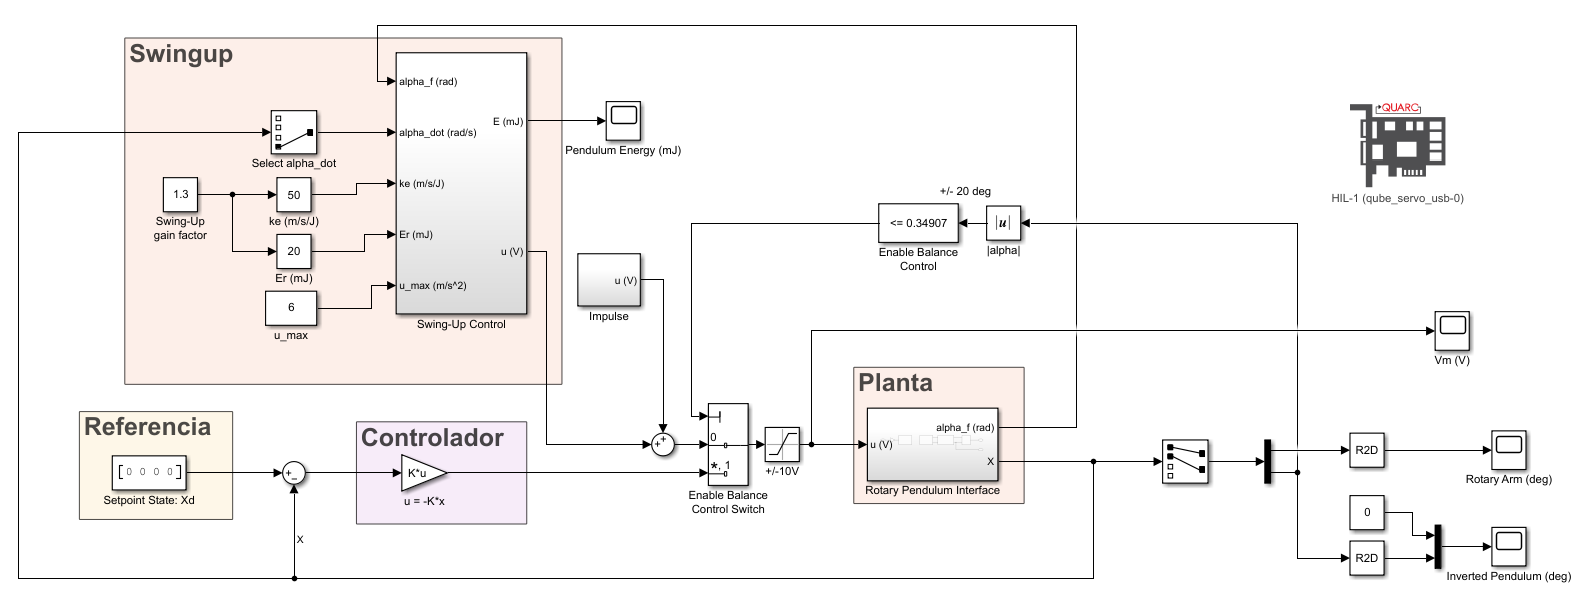
\includegraphics[width=\textwidth]{images/simulink_act3.png}
    \caption{Diagrama de bloques de la Actividad 3 en Simulink.}
    \label{fig:actividad3_diagrama}
\end{figure}
En su explicación, describa la función general del sistema de \textbf{swing-up}, la función de los bloques del diagrama principal y del subsistema \textbf{Swing-Up Control}, el cálculo de la \textbf{energía del péndulo} y la lógica del bloque \textbf{Enable Balance Control} para el cambio entre swing-up y balanceo LQR. \\
Además, presente las siguientes gráficas:
\begin{itemize}
        \item Comportamiento del brazo rotatorio: $\theta$
        \item Control del péndulo invertido: $\alpha$ vs. $\alpha_{\text{deseado}}$
        \item Esfuerzo de control: Voltaje
    \item Energía del péndulo
\end{itemize}

\noindent A diferencia de las actividades anteriores, en esta implementación ya no es necesario colocar manualmente el péndulo cerca de la posición invertida para que el controlador LQR pueda estabilizarlo. El algoritmo \textit{swing-up} permite iniciar el sistema desde la posición colgante natural del péndulo, inyectando progresivamente energía mediante movimientos oscilatorios del brazo rotatorio hasta llevar el péndulo a la región cercana de la posición invertida.

\noindent El funcionamiento general puede interpretarse como una lógica condicional de cambio de control. Mientras el péndulo se encuentra lejos de la posición invertida, permanece activo el controlador \textit{swing-up}, encargado de incrementar la energía del sistema para “columpiar” el péndulo. Una vez que el ángulo y la energía alcanzan un rango cercano al equilibrio invertido, el bloque \textbf{Enable Balance Control} habilita automáticamente el controlador LQR y desactiva el swing-up. A partir de ese instante, el LQR toma el control del sistema y mantiene el péndulo estabilizado alrededor de la posición invertida con pequeñas oscilaciones.


% --- Comportamiento del brazo rotatorio ---
\begin{figure}[H]
    \centering
    
\includegraphics[width=0.85\textwidth]{A3/theta.png}
    \caption{Comportamiento del brazo rotatorio $\theta$ durante el swing-up y el balanceo LQR.}
    \label{fig:act3_theta}
\end{figure}
\noindent Durante la fase de swing-up, el brazo $\theta$ realiza movimientos oscilatorios crecientes que inyectan energía al péndulo mediante  controlado. Una vez que el péndulo alcanza la zona cercana a la posición invertida y se activa el controlador LQR, el brazo se estabiliza alrededor de $\theta = 0$ rad, manteniéndose dentro de un rango pequeño.

% --- Control del péndulo invertido ---
\begin{figure}[H]
    \centering
    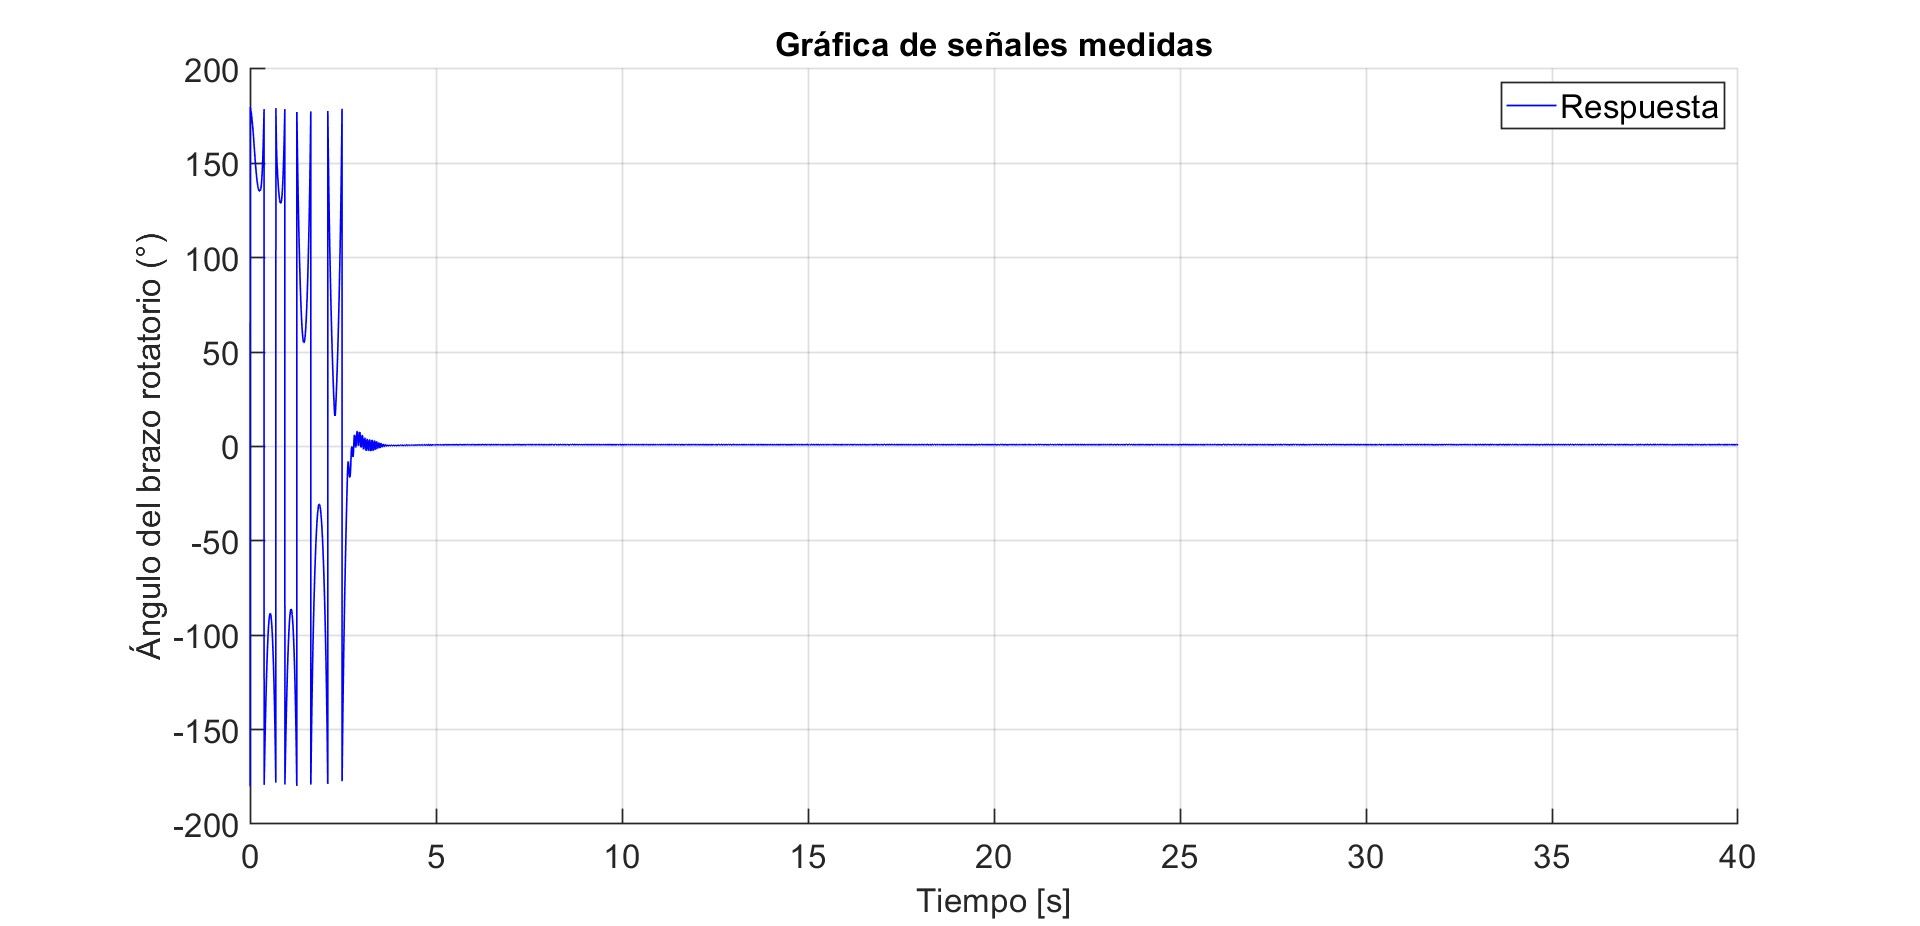
\includegraphics[width=0.85\textwidth]{images/Figura_24.jpg}
    \caption{Control del péndulo invertido: $\alpha$ vs. $\alpha_{\text{deseado}}$.}
    \label{fig:act3_alpha}
\end{figure}

% --- Esfuerzo de control: voltaje ---
\begin{figure}[H]
    \centering
    
\includegraphics[width=0.85\textwidth]{A3/voltaje.png}
    \caption{Esfuerzo de control: voltaje $V_m$ aplicado al motor.}
    \label{fig:act3_voltaje}
\end{figure}
\noindent Durante el swing-up, el voltaje $V_m$ presenta una forma alternada característica del bombeo de energía: el algoritmo aplica voltaje en la dirección del movimiento del péndulo para incrementar su energía mecánica. Tras la conmutación al controlador LQR, la señal de voltaje pasa a ser una corrección suave de baja amplitud, propia del régimen de balanceo en torno al punto de equilibrio.

% --- Energía del péndulo ---
\begin{figure}[H]
    \centering
    
\includegraphics[width=0.85\textwidth]{A3/energia.png}
    \caption{Energía del péndulo $E$ durante la ejecución del algoritmo swing-up.}
    \label{fig:act3_energia}
\end{figure}
\noindent La Figura~\ref{fig:act3_energia} evidencia el principio de funcionamiento del algoritmo \textit{swing-up}, basado en el control de energía del péndulo. Inicialmente, la energía es baja debido a que el péndulo se encuentra en reposo en la posición colgante. Conforme el brazo oscila, el controlador incrementa progresivamente la energía total del sistema hasta aproximarse al nivel energético correspondiente a la posición invertida. Cuando esta condición es alcanzada y el péndulo se encuentra dentro del rango angular permitido, el bloque \textbf{Enable Balance Control} conmuta automáticamente del controlador swing-up al controlador LQR para realizar el balanceo estable.